\subsection{空间与单连通空间的积}

命题 8. —— 设 B 为拓扑空间，T 为单连通且局部连通的空间，E 为 B × T 的覆叠，其投影为 p，并设 t 为 T 的一点。以 \(E_{t}\) 表示空间 \(p^{-1}(B \times \{t\})\) ，它带有映射 \(p_{t} = pr_{1} \circ p \mid E_{t}: E_{t} \to B\) ；这是 B 的一个覆叠。则存在唯一的从覆叠 ( \(E_{t} \times T, p_{t} \times Id_{T}\) ) 到覆叠 E 上的 (B × T)-同构，它把每个 \(x \in E_{t}\) 的 (x, t) 映为 x 。

可以假设 B 非空。设 \(x\) 为 \(E_t\) 的一点。把 I, 第 125 页命题 3 应用于覆叠 E 和连续映射 T → B × T, \(u \mapsto (p_t(x), u)\) ，便存在唯一的连续映射 \(f_x \colon \mathrm{T} \to \mathrm{E}\) ，使得 \(f_x(t) = x\) 且 \(p(f_x(u)) = (p_t(x), u)\) 对所有 \(u \in T\) 成立。设 \(h \colon E_t \times T \to E\) 为由 \(h(x, u) = f_x(u)\) 定义的映射。我们有 \(h(x, t) = x\) 与 \(p \circ h = p_t \times \operatorname{Id}_T\) 。映射 h 是映射 \(p_t \times \operatorname{Id}_T\) 到 E 中的提升。h 在 \(E_t \times \{t\}\) 上的限制是连续的，h 在 \(\{x\} \times T\) 上的限制对 \(E_t\) 的每一点 x 也是连续的。由于空间 T 局部连通，映射 h 连续（I, 第 37 页, 定理 1 的推论 1）。

设 \(b\) 为 B 的一点。按构造，映射 \(h\) 诱导从纤维 \(p_t^{-1}(b) \times \{t\}\) （\(E_t \times T\) 的纤维）到纤维 \(p^{-1}(b,t)\) （E 在点 \((b,t)\) 处的纤维）上的双射。由于空间 T 连通且局部连通，映射 \(h\) 是双射（I, 第 84 页, 命题 7 的推论）。因此它是 \(B \times T\) -同构（I, 第 30 页, 命题 6 的推论 2）。

设 \(h'\) 为一个 \((\mathrm{B} \times \mathrm{T})\) -同构，它从覆叠 \((\mathrm{E}_{t} \times \mathrm{T}, p_{t} \times \mathrm{Id}_{\mathrm{T}})\) 映到覆叠 E 上，且把 \((x, t)\) 映为 x（对每一点 \(x \in E_{t}\) ）。对所有 \(x \in E_{t}\) ，映射 \(u \mapsto h(x, u)\) 与 \(u \mapsto h'(x, u)\) 相等（I, 第 34 页, 命题 11 的推论 1）。于是有 \(h = h'\) 。

推论 1. —— 在命题 8 的假设下，若 t 与 t' 为 T 的两点，则覆叠 \(E_{t}\) 与 \(E_{t'}\) 是 B-同构的。

推论 2. —— 在命题 8 的假设下，设 (E,p) 与 (E',p') 为 B × T 的覆叠，并设 \(k: E_t \to E_t'\) 为 B-态射。则存在唯一的 (B × T)-态射 \(\widetilde{k}\) : E → E'，它扩张 k。若 k 是 B-同构，则 \(\widetilde{k}\) 是 (B × T)-同构。

由命题 8，可以假设存在 B 的覆叠 F 与 F′，使得 E 与 E′ 分别为 (B × T)-空间 F × T 与 F′ × T。于是有 \(E_{t} = F \times \{t\}\) ，\(E_{t}' = F' \times \{t\}\) ，且映射 k 写作 \((x, t) \mapsto (k'(x), t)\) ，其中 \(k'\) 是从 F 到 F' 中的 B-态射。映射 \(k' \times Id_{T}\) 是扩张 k 的 B × T-态射；若 k 是同构，则它也是同构。

设 \(\widetilde{k}\colon\mathrm{E}\to\mathrm{E}^{\prime}\) 为 \((\mathrm{B}\times\mathrm{T})\) -态射，它扩张 \(k\) 。设 \(x\) 为 F 的一点。以 \(q\) 表示 F 的投影，并令 \(b=q(x)\) 。映射 \(u\mapsto\widetilde{k}(x,u)\) 与 \(u\mapsto(k^{\prime}(x),u)\) 是在 \(\mathrm{E}^{\prime}\) 中的提升，所提升的映射为 \(u\mapsto(b,u)\) ，它把 T 映到 \(\mathrm{B}\times\mathrm{T}\) 。它们在 \(t\) 处相合。由于空间 T 连通，它们相等。于是，\(\widetilde{k}\) 就是 \((\mathrm{B}\times\mathrm{T})\) -态射 \(k^{\prime}\times\mathrm{Id}_{\mathrm{T}}\colon\mathrm{F}\times\mathrm{T}\to\mathrm{F}^{\prime}\times\mathrm{T}\) 。

推论 3. —— 设 B 与 B' 为拓扑空间，T 为单连通且局部连通的拓扑空间。设 \(f: B' \times T \to B\) 为连续映射，E 为 B 的覆叠。给定 T 的一点 t 和一个连续提升 \(g_t: B' \times \{t\} \to E\) （\(f | B' \times \{t\}\) 到 E 中的提升），存在唯一的 f 到 E 中的连续提升 g，它扩张 \(g_t\) 。

由 I, 第 9 页命题 3，只需证明 \(f^{*}(\mathrm{E})\) 在 \(\mathrm{B}' \times \{t\}\) 上的每个连续截面都唯一地扩张为 \(f^{*}(\mathrm{E})\) 的连续截面。而这由把推论 2 应用于覆叠 \((\mathrm{B}' \times \mathrm{T}, \mathrm{Id}_{\mathrm{B}' \times \mathrm{T}})\) 与 \(f^{*}\mathrm{E}\) （二者都是 \(\mathrm{B}' \times \mathrm{T}\) 的覆叠）即得。

注. —— 保留命题 8 的假设与记号。设 G 为离散拓扑群。假设 E 是以 G 为群的主覆叠。若给覆叠 \(E_{t}\) （B 的）与覆叠 \(E_{t} \times T\) （\(B \times T\) 的）赋予由 E 的结构导出的以 G 为群的主覆叠结构（I, 第 92 页, 例 1 与例 4），则覆叠 E 与 \(E_{t} \times T\) 是同构的主覆叠。事实上，设 \(h: E_{t} \times T \to E\) 为唯一的 (B × T)-态射，使得 \(h(x, t) = x\) （对所有 \(x \in E_{t}\) ）。对 G 的每个元素 g，映射 \((x, u) \mapsto h(x \cdot g, u) \cdot g^{-1}\) 是把 \((x, t)\) （对所有 \(x \in E_{t}\) ）映为 x 的 (B × T)-态射，因此等于 h。这就证明了 h 是主覆叠的 (B × T)-态射。

特别地，在前述假设之下，主覆叠 \(E_{t}\) 与 \(E_{t'}\) （对 \(t' \in T\) ）是同构的。类似地可以证明：若在推论 2 中 E 与 \(E'\) 是以 G 为群的主覆叠，且 k 是以 G 为群的主覆叠的 B-同构，则 \(\widetilde{k}\) 是主覆叠的 \((\mathrm{B} \times \mathrm{T})\) 同构。

命题 9. —— 设 B 为拓扑空间，(E,p) 为 B 的覆叠。设 T 为单连通、局部连通且局部紧的拓扑空间。以 \(\widetilde{p}\colon\mathcal{C}_{c}(\mathrm{T};\mathrm{E})\to\mathcal{C}_{c}(\mathrm{T};\mathrm{B})\) 表示映射 \(g\mapsto p\circ g\) 。设 t 为 T 的一点。以 \(e_{\mathrm{E}}\colon\mathcal{C}_{c}(\mathrm{T};\mathrm{E})\to\mathrm{E}\) 表示把每个 \(g\in\mathcal{C}_{c}(\mathrm{T};\mathrm{E})\) 对应到 \(g(t)\) 的映射，以 \(e_{\mathrm{B}}\colon\mathcal{C}_{c}(\mathrm{T};\mathrm{B})\to\mathrm{B}\) 表示把每个 \(f\in\mathcal{C}_{c}(\mathrm{T};\mathrm{B})\) 对应到 \(f(t)\) 的映射。

方块

\[
\begin{array}{c} \mathcal {C} _ {c} (\mathrm{T}; \mathrm{E}) \xrightarrow {e _ {\mathrm{E}}} \mathrm{E} \\ \Big \downarrow \widetilde {p} \\ \mathcal {C} _ {c} (\mathrm{T}; \mathrm{B}) \xrightarrow {e _ {\mathrm{B}}} \mathrm{B} \end{array}
\]

是笛卡尔的。

我们先证明一个引理。

引理. —— 设 X, Y, Z 为拓扑空间，\(g: Y \rightarrow Z\) 为连续映射。

\begin{enumerate}
\def\labelenumi{\alph{enumi})}
\item
  映射 \(f\mapsto g\circ f\) （从 \(\mathcal{C}_c(\mathrm{X};\mathrm{Y})\) 到 \(\mathcal{C}_c(\mathrm{X};\mathrm{Z})\) ）是连续的。
\item
  若拓扑空间 Z 是豪斯多夫的，则映射 \(h \mapsto h \circ g\) （从 \(\mathcal{C}_{c}(\mathrm{Z};\mathrm{X})\) 到 \(\mathcal{C}_{c}(\mathrm{Y};\mathrm{X})\) ）是连续的。
\end{enumerate}

给定 X 的紧子集 K、Z 的开子集 U 以及从 X 到 Y 的连续映射 f，要有 \((g \circ f)(\mathrm{K}) \subset \mathrm{U}\) ，必须且只需 \(f(\mathrm{K}) \subset g^{-1}(\mathrm{U})\) 。因此第一个断言由紧收敛拓扑的定义得出（TG, X, 第 26 页, 定义 1）。

类似地，设 K 为 Y 的紧子集，U 为 X 的开子集。由于假设空间 Z 是豪斯多夫的，集合 \(g(\mathrm{K})\) 是紧的（TG, I, 第 63 页, 推论 1）。若 h 是从 Z 到 X 中的一个映射，则条件 \((h \circ g)(\mathrm{K}) \subset \mathrm{U}\) 无非就是条件 \(h(g(\mathrm{K})) \subset \mathrm{U}\) ，由此得出第二个断言。

现在来证明命题 9。由引理，映射 \(\widetilde{p}\) 连续；由 TG, X, 第 27 页的注 1，映射 \(e_{\mathrm{E}}\) 与 \(e_{\mathrm{B}}\) 连续。对任意映射 \(g \in \mathcal{C}_c(\mathrm{T};\mathrm{E})\) ，我们有

\[
(p \circ e _ {\mathrm{E}}) (g) = p (g (t)) = (p \circ g) (t) = \widetilde {p} (g) (t) = \left(e _ {\mathrm{B}} \circ \widetilde {p}\right) (g),
\]

于是命题中的方块图是交换的。

设 \(\varphi\colon\mathcal{C}_{c}(\mathrm{T};\mathrm{E})\to\mathcal{C}_{c}(\mathrm{T};\mathrm{B})\times_{\mathrm{B}}\mathrm{E}\) 为由 \(\varphi(g)=(p\circ g,g(t))\) （对所有 \(g\in\mathcal{C}_{c}(\mathrm{T};\mathrm{E})\) ）定义的连续映射。由 I, 第 125 页命题 3，它是双射。事实上，对每一对 \((f,x)\in\mathcal{C}_{c}(\mathrm{T};\mathrm{B})\times_{\mathrm{B}}\mathrm{E},\varphi^{-1}(f,x)\) 是到 E 中的唯一连续提升 \(g\) （它提升 \(f\) ），使得 \(g(t)=x\) 。由于空间 T 局部紧，映射 \(\psi\colon(\mathcal{C}_{c}(\mathrm{T};\mathrm{B})\times_{\mathrm{B}}\mathrm{E})\times\mathrm{T}\to\mathrm{B}\) （由 \(\psi((f,x),u)=f(u)\) 定义）是连续的（TG, X, 第 28 页, 推论 1）。由前面的推论 3，映射 \(\psi\) 有唯一的连续提升 \(\theta\colon(\mathcal{C}_{c}(\mathrm{T};\mathrm{B})\times_{\mathrm{B}}\mathrm{E})\times\mathrm{T}\to\mathrm{E}\) ，使得 \(\theta((f,x),t)=x\) （对 \((f,x)\in\mathcal{C}_{c}(\mathrm{T};\mathrm{B})\times_{\mathrm{B}}\mathrm{E}\) ）。于是有 \(\theta((f,x),u)=\varphi^{-1}(f,x)(u)\) （对 \((f,x)\in\mathcal{C}_{c}(\mathrm{T};\mathrm{B})\times_{\mathrm{B}}\mathrm{E}\) 与 \(u\in\mathrm{T}\) ）。由 TG, X, 第 28 页定理 3，映射 \((f,x)\mapsto\theta((f,x),\cdot)\) （从 \(\mathcal{C}_{c}(\mathrm{T};\mathrm{B})\times_{\mathrm{B}}\mathrm{E}\) 到 \(\mathcal{C}_{c}(\mathrm{T};\mathrm{E})\) ）是连续的，也就是说 \(\varphi^{-1}\) 连续。

这样，映射 \(\varphi\) 就是从 \(\mathcal{C}_c(\mathrm{T};\mathrm{E})\) 到纤维积 \(\mathcal{C}_c(\mathrm{T};\mathrm{B})\times_{\mathrm{B}}\mathrm{E}\) 上的同胚，由此即得命题（I, 第 8 页, 命题 2）。

\subsection{单连通空间的同胚群}

设 X 为非空连通拓扑空间，G 为从左边连续作用于 X 的离散群；以 e 表示 G 的单位元。设 M 为 X 的子集，使得 \(G \cdot M = X\) 。我们令

\[
\mathrm{S} = \{g \in \mathrm{G} \mid g \cdot \mathrm{M} \cap \mathrm{M} \neq \varnothing \}.
\]

我们有 \(e \in S\) 且 \(S = S^{-1}\) 。

对每个 \(x \in X\) ，以 \(E_{x}\) 表示这样的 \(g \in G\) 所成的集：\(x \in g \cdot M\) 。设 \(g, h \in E_{x}\) ；则 \(g \cdot M \cap h \cdot M \neq \varnothing\) ，从而 \(g^{-1}h \in S\) 。特别地，对每个 \(x \in M\) ，我们有 \(e \in E_{x}\) ，于是 \(E_{x} \subset S\) 。

我们作下列两个假设之一：

\begin{enumerate}
\def\labelenumi{(\roman{enumi})}
\item
  集合 M 是开集；
\item
  集合 M 是闭集，且 X 的覆盖 \((g \cdot \mathrm{M})_{g \in \mathrm{G}}\) 是局部有限的。
\end{enumerate}

引理 2. —— 对每一点 \(x \in X\) ，映射 \(\mu_x: E_x \times M \to X\) （由 \((g, u) \mapsto g \cdot u\) 给出）是普遍严格的，且其像 \(E_x \cdot M\) 是 \(x\) 在 \(X\) 中的一个邻域。特别地，\(S \cdot M\) 是 \(M\) 的一个邻域。

在假设 (i) 之下，映射 \(\mu_{x}\) 是开的，因为 \(E_{x} \times M\) 在 \(G \times M\) 中是开集。于是其像在 X 中是开集。

现在假设 (ii) 成立。映射 \(\mu_x\) 是逆紧的（TG, I, 第 6 页, 命题 4, 以及第 75 页, 定理 1），因而是普遍严格的（I, 第 20 页, 推论 11）。此外，\((\mathrm{G} - \mathrm{E}_x) \cdot \mathrm{M}\) 是 X 的不包含 \(x\) 的闭子集，因此 \(\mathrm{E}_x \cdot \mathrm{M}\) 是 \(x\) 的一个邻域。

最后一个断言由如下事实得出：\(E_{x} \subset S\) （若 \(x \in M\) ）。

引理 3. —— 群 G 由 S 生成。

设 H 为 G 的由 S 生成的子群。令 U = H·M ；注意 U 是形如 \(h \cdot (S \cdot M)\) （\(h \in H\) ）的子集的并。由于 S · M 是 M 的一个邻域（引理 2），集合 U 是 H · M = U 的一个邻域；由此可知 U 在 X 中是开集。设 \(g, g' \in G\) 使得 \(g \cdot U \cap g' \cdot U \neq \varnothing\) ；设 \(h, h' \in H\) 与 \(x, x' \in M\) 使得 \(gh \cdot x = g'h' \cdot x'\) ；则 \(h^{-1}g^{-1}g'h' \cdot x' = x\) ，从而 \(h^{-1}g^{-1}g'h' \in S\) ；特别地，\(g^{-1}g' \in H\) 。当 \(g\) 取遍模 \(H\) 的左陪集的代表系时，诸集合 \(g \cdot U\) 两两不交；由于 \(G \cdot M = X\) ，它们覆盖 \(X\) 。由于 \(X\) 连通，由此得出 \((G : H) = 1\) ，从而 \(H = G\) 。

设 T 为 G 中元素之对 \((s,t)\) 所成的集，使得 \(M\cap s\cdot M\cap st\cdot M\neq\varnothing\) ；若 \((s,t)\in\mathrm{T}\) ，则 s、t 与 st 都属于 S。设 F 为群 \(\mathrm{F}(\mathrm{S},\mathbf{r})\) ，它由生成元集 S 与关系元 \(str^{-1}\) （对 \(r,s,t\in S\) ，满足 \((s,t)\in\mathrm{T}\) 且 r=st）所成的集 r 定义；以 \(\varepsilon\) 表示其单位元，以 \(\varphi\colon F\to G\) 表示典范同态（A, I, 第 86 页, 命题 9）。若 \(s\in S\) ，我们将以 \(x_{s}\) 表示 F 中的元素，即 s 在从 S 到 F 的典范映射下的像；对每个 \(s\in S\) ，有 \(\varphi(x_{s})=s\) 。于是同态 \(\varphi\) 是满射的（引理 3）。对 \((s,t)\in\mathrm{T}\) 与 r=st，有 \(x_{r}=x_{s}x_{t}\) ；从而有 \(x_{e}=\varepsilon\) ，因为 \((e,e)\in\mathrm{T}\) ；对每个 \(s\in S\) ，还有 \(x_{s^{-1}}=x_{s}^{-1}\) ，因为 \((s,s^{-1})\in\mathrm{T}\) 。

给集合 F 赋予离散拓扑，并以 Z 表示拓扑空间 \(F \times M\) ，它带有由 \((\gamma, (g, x)) \mapsto (\gamma g, x)\) （对 \(\gamma\) 与 \(g \in F\) 以及 \(u \in M\) ）给出的 F 的作用。设 \((g_{1}, u_{1})\) 与 \((g_{2}, u_{2})\) 为 Z 的元素；我们说 \((g_{1}, u_{1})\) 与 \((g_{2}, u_{2})\) 同余，如果存在 \(s \in S\) 使得 \(g_{2} = g_{1} \cdot x_{s}\) 且 \(s \cdot u_{2} = u_{1}\) 。

引理 4. —— 关系“ \((g_{1}, u_{1})\) 与 \((g_{2}, u_{2})\) 同余”是 Z 上的一个等价关系，且与 F 的作用相容。

这个关系是自反的，因为我们有 \(x_e = \varepsilon\) 。设 \((g_1, u_1)\) 与 \((g_2, u_2)\) 为 Z 的元素，使得 \((g_1, u_1)\) 与 \((g_2, u_2)\) 同余。设 \(s \in S\) 使得 \(g_2 = g_1 x_s\) 且 \(s \cdot u_2 = u_1\) ；由于 \(x_{s^{-1}} = x_s^{-1}\) ，我们有 \(g_1 = g_2 x_{s^{-1}}\) 与 \(u_2 = s^{-1} \cdot u_1\) ，因此 \((g_2, u_2)\) 与 \((g_1, u_1)\) 同余；从而这个关系是对称的。最后来证明它是传递的。设 \((g_1, u_1)\) 、\((g_2, u_2)\) 与 \((g_3, u_3)\) 为 Z 的点，使得 \((g_1, u_1)\) 与 \((g_2, u_2)\) 同余，\((g_2, u_2)\) 与 \((g_3, u_3)\) 也同余。设 \(s\) 与 \(t\) 属于 S，使得一方面 \(g_2 = g_1 x_s\) 且 \(s \cdot u_2 = u_1\) ，另一方面 \(g_3 = g_2 x_t\) 且 \(t \cdot u_3 = u_2\) 。我们有 \(u_1 = s \cdot u_2 = st \cdot u_3\) ，因此 \(u_1 \in M \cap s \cdot M \cap st \cdot M\) ，这表明 \((s, t)\) 属于 T 且 \(st\) 属于 S。于是有 \(g_3 = g_2 x_t = g_1 x_s x_t = g_1 x_{st}\) 与 \(u_1 = st \cdot u_3\) ，因此 \((g_1, u_1)\) 与 \((g_3, u_3)\) 同余。这样一来，“同余”关系就是 Z 上的一个等价关系。它与 F 在 Z 上的作用相容。

设 Y 为 Z 关于上述等价关系的商拓扑空间。以 \(\pi\colon\mathrm{Z}\to\mathrm{Y}\) 表示典范映射。

我们还以 \(q \colon \mathrm{Z} \to \mathrm{X}\) 表示由 \((g, x) \mapsto \varphi(g) \cdot x\) 给出的映射；它是满射的（引理 3）。通过取商，映射 \(q\) 诱导一个连续且满射的映射 \(p \colon \mathrm{Y} \to \mathrm{X}\) ；由引理 4，F 在 Z 上的作用诱导 F 在 Y 上的一个连续作用，使得 \(p(g \cdot y) = \varphi(g) \cdot p(y)\) （对所有 \(g \in \mathrm{F}\) 与每一点 \(y \in \mathrm{Y}\) ）。特别地，群 \(\mathrm{N} = \mathrm{Ker}(\varphi)\) 连续地作用于 X-空间 \((\mathrm{Y}, p)\) 。

引理 5. —— 若 M 连通，则空间 Y 连通。

设 \(g \in F\) 与 \(s \in S\) 。设 u 与 v 为 M 的元素，使得 \(v = s \cdot u\) ；于是有 \(\pi(g, v) = \pi(gx_s, u)\) ，且 Y 的集合 \(\pi(\{g\} \times M)\) 与 \(\pi(\{gx_s\} \times M)\) 有一个公共点。由于它们都是连通的，它们含于 Y 的同一个连通分支。由于 S 是群 G 的对称子集，且 \(x_{s^{-1}} = x_s^{-1}\) （对所有 \(s \in S\) ），F 的每个元素 g 都形如 \(x_{s_1} \ldots x_{s_n}\) ，其中 \(n \in \mathbb{N}\) 且 \(s_1, \ldots, s_n\) 是 S 的元素。对 n 用归纳法，集合 \(\pi(\{e\} \times M)\) 与 \(\pi(\{g\} \times M)\) （对每个 \(g \in F\) ）含于 Y 的同一个连通分支。由此得出 Y 是连通的。

引理 6. —— 对每个 \(x \in X\) ，群 N 忠实且传递地作用于纤维 \(p^{-1}(x)\) 上。

由于 \(p\) 是满射的，纤维 \(p^{-1}(x)\) 非空。设 \(y, y' \in p^{-1}(x)\) ；我们来证明存在唯一的元素 \(n \in \mathrm{N}\) 使得 \(n \cdot y = y'\) 。设 \(g, h \in \mathrm{F}\) ，并设 \(u, v \in \mathrm{M}\) 使得 \(y = \pi(g, u)\) 与 \(y' = \pi(h, v)\) 。令 \(s = \varphi(g^{-1}h)\) 。由于 \(x = \varphi(g) \cdot u = \varphi(h) \cdot v\) ，我们有 \(u = s \cdot v\) ，从而 \(s \in \mathrm{S}\) 。由此得出 \(\varphi(h) = \varphi(gx_s)\) ，因此存在 \(n \in \mathrm{N}\) 使得 \(h = ngx_s\) 。于是，

\[
y ^ {\prime} = \pi (h, v) = \pi (n g x _ {s}, v) = n \cdot \pi (g x _ {s}, v) = n \cdot \pi (g, s \cdot v) = n \cdot y.
\]

设 \(n'\) 为 N 的元素，使得 \(n' \cdot y = y'\) 。我们有 \(n' \cdot \pi(g, u) = n \cdot \pi(g, u)\) ，从而 \(\pi(n'g, u) = \pi(ng, u)\) 。因此，存在 \(t \in S\) 使得 \(n'g = ngx_t\) ；这个关系蕴含 \(\varphi(x_t) = e\) ，从而 \(t = e\) 且 \(n = n'\) 。

引理 7. —— 赋有 N 的作用的 X-空间 (Y,p) 是一个左主覆叠。它在 M 上是可平凡化的。

设 \(x \in \mathrm{X}\) ；我们取定一个元素 \(g \in \mathrm{E}_x\) 以及一个元素 \(\overline{g} \in \mathrm{F}\) 使得 \(\varphi(\overline{g}) = g\) 。以 \(\mu_x \colon \mathrm{E}_x \times \mathrm{M} \to \mathrm{X}\) 表示由 \((h, u) \mapsto h \cdot u\) 给出的映射。

设 \(n \in \mathrm{N}\) ，设 \(h, k \in \mathrm{E}_x\) ，并设 \(u, v \in \mathrm{M}\) 使得 \(h \cdot u = k \cdot v\) ；令 \(s = g^{-1}h\) ，\(t = h^{-1}k\) 与 \(r = st = g^{-1}k\) 。由于 \(x\) 属于 \(g \cdot M \cap h \cdot M \cap k \cdot M\) ，对 \((s, t)\) 属于 T，从而 \(x_s x_t = x_r\) 。于是我们有

\[
\pi (n \overline {{g}} x _ {r}, v) = \pi (n \overline {{g}} x _ {s} x _ {t}, v) = \pi (n \overline {{g}} x _ {s}, t \cdot v) = \pi (n \overline {{g}} x _ {s}, u).
\]

于是存在唯一的映射 \(\theta\colon\mathrm{N}\times(\mathrm{E}_{x}\cdot\mathrm{M})\to\mathrm{Y}\) ，使得 \(\theta(n,h\cdot u)=\pi(n\overline{g}x_{g^{-1}h},u)\) （对所有 \(n\in\mathrm{N}\) 、所有 \(h\in\mathrm{E}_{x}\) 与每个 \(u\in\mathrm{M}\) ）。我们有

\[
p (\theta (n, h \cdot u)) = p (\pi (n \overline {{g}} x _ {s}, u)) = q (n \overline {{g}} x _ {s}, u) = \varphi (n \overline {{g}} x _ {s}) \cdot u = g s \cdot u = h \cdot u.
\]

此外，对 \(n, n' \in \mathrm{N}\) 与 \(y \in \mathrm{E}_x \cdot \mathrm{M}\) ，我们有 \(\theta(n'n, y) = n' \cdot \theta(n, y)\) 。映射 \(\theta'\colon \mathrm{N} \times (\mathrm{E}_x \times \mathrm{M}) \to \mathrm{Y}\) （由 \(\theta'(n, (h, u)) = \theta(n, \mu_x(h, u))\) 给出）是连续的；由于映射 \(\mu_x\) 是普遍严格的（I, 第 133 页, 引理 2），映射 \(\theta\) 连续。它是从 \(\mathrm{N} \times (\mathrm{E}_x \cdot \mathrm{M})\) 到 Y 的子空间 \(\mathrm{Y} \times_{\mathrm{X}} (\mathrm{E}_x \cdot \mathrm{M})\) 上的双射（引理 6）。

设 \(z = (\overline{k}, v) \in \mathbf{Z}\) 与 \((h, u) \in \mathrm{E}_x \times \mathrm{M}\) 使得 \(q(\overline{k}, v) = \mu_x(h, u)\) 。令 \(s = h^{-1}\varphi(\overline{k})\) ；由于 \(\varphi(\overline{k}) \cdot v = h \cdot u\) ，我们有 \(s \in S\) 。于是令 \(\lambda'(z, (h, u)) = \overline{k} x_s^{-1} x_{h^{-1}g} \overline{g}^{-1}\) ；我们有 \(\varphi(\lambda'(z, (h, u))) = \varphi(\overline{k}) s^{-1} h^{-1} gg^{-1} = e\) ，因此 \(\lambda'(z, (h, u)) \in \mathrm{N}\) 。这样就定义了一个连续映射 \(\lambda' \colon \mathbf{Z} \times_{\mathbf{X}} (\mathrm{E}_x \times \mathrm{M}) \to \mathrm{N}\) 。而且，对如上所述的每个 \(z\) 与 \((h, u)\) ，有

\[
\begin{array}{r l} & {\theta (\lambda^ {\prime} (z, (h, u)), h \cdot u) = \pi (\overline {{k}} x _ {s} ^ {- 1} x _ {h ^ {- 1} g} \overline {{g}} ^ {- 1} \overline {{g}} x _ {g ^ {- 1} h}, u)} \\ & {\qquad = \pi (\overline {{k}} x _ {s} ^ {- 1}, u) = \pi (\overline {{k}}, s ^ {- 1} \cdot u) = \pi (\overline {{k}}, v) = \pi (z),} \end{array}
\]

且 \(\lambda'(z,(h,u))\) 是 N 中唯一的元素 \(n\) ，使得 \(\theta(n,h\cdot u)=\pi(z)\) 。特别地，存在唯一的映射

\[
\lambda \colon Y \times_ {X} (E _ {x} \cdot M) \to N
\]

使得 \(\lambda(\pi(z), h \cdot u) = \lambda'(z, (h, u))\) （对所有 \(z \in \mathbf{Z}\) 与每个 \((h, u) \in \mathrm{E}_x \times \mathrm{M}\) ，满足 \(q(z) = h \cdot u\) ）。它是连续的，因为映射 \(\mu_x\) 是普遍严格的。由此得出，由 Y 换基而得的 \(\mathrm{E}_x \cdot \mathrm{M}\) -空间 \(\mathrm{Y}_{\mathrm{E}_x \cdot \mathrm{M}}\) ，赋有 N 的作用，是一个以 N 为群的主纤维丛，并且是可平凡化的。

引理证毕。

命题 10. —— 设 X 为非空连通拓扑空间，G 为从左边连续作用于 X 的离散群，M 为 X 的子集且 G · M = X。作下列两个假设之一：

\begin{enumerate}
\def\labelenumi{(\roman{enumi})}
\item
  集合 M 是开集；
\item
  集合 M 是闭集，且 X 的覆盖 \((g \cdot \mathrm{M})_{g \in \mathrm{G}}\) 是局部有限的。
\end{enumerate}

设 S 为由元素 \(g \in G\) （满足 \(M \cap g \cdot M \neq \varnothing\) ）所成的集，T 为由对 \((s, t) \in S \times S\) （满足 \(M \cap s \cdot M \cap st \cdot M \neq \varnothing\) ）所成的集。设 F 为群 \(F(S, r)\) ，它由生成元集 S 与关系元 \(str^{-1}\) （对 \(r, s, t \in S\) ，满足 \((s, t) \in T\) 且 r = st）所成的集 r 定义；对 \(s \in S\) ，以 \(x_s\) 表示 s 在从 S 到 F 的典范映射下的像。存在唯一的群同态 \(\varphi: F \to G\) ，使得 \(\varphi(x_s) = s\) （对所有 \(s \in S\) ）。它是满射的；若空间 X 单连通，或者更一般地，若 X 的每个在 M 上可平凡化的覆叠都是可平凡化的，则它是同构。

同态 \(\varphi\) 是满射的（I, 第 133 页, 引理 3）。用刚才引进的记号，X 的覆叠 Y 是可平凡化的，因为它在 M 上可平凡化。由引理 5，Y 连通。因此，\(p\colon\mathrm{Y}\to\mathrm{X}\) 是同胚且群 N 化为单位元。于是，同态 \(\varphi\colon\mathrm{F}\to\mathrm{G}\) 是群同构。

命题 11. —— 设 X 为单连通拓扑空间，G 为从右边连续作用于 X 的离散群。若 G 的由 X 各点的稳定子群之并所生成的子群等于 G，则空间 X/G 是单连通的。

设 (E, p) 为 X/G 的覆叠。我们需要证明，对 E 的每一点 x，存在 p 的连续截面 s 使得 \(s \circ p(x) = x\) （I, 第 70 页, 命题 1 的推论 2）。以 \(q: X \to X/G\) 表示典范映射，并选取 X 的一点 y 使得 \(q(y) = p(x)\) 。由于空间 X 单连通，存在连续映射 \(f: X \to E\) 使得 \(f(y) = x\) 且 \(p \circ f = q\) （I, 第 125 页, 命题 3）。设 z 为 X 的一点，g 为固定 z 的 G 的那个子群的元素。从 X 到 E 中的映射 \(t \mapsto f(t)\) 与 \(t \mapsto f(t \cdot g)\) 是映射 q 到 E 中的连续提升，且它们在 t = z 处相合。由于空间 X 连通，它们相等（I, 第 34 页, 命题 11 的推论 1）。由于 X 各点的稳定子群之并生成 G，我们有 \(f(t \cdot g) = f(t)\) （对所有 \(t \in X\) 与每个 \(g \in G\) ）。通过取商，我们从 f 导出连续映射 s: X/G → E，它是 p 的连续截面且满足 \(s(p(x)) = x\) 。

\exerciseshdr{习题}

\exercisegroup

\begin{enumerate}
\def\labelenumi{\arabic{enumi})}
\tightlist
\item
  设 B 为拓扑空间，\((X,p)\) 与 \((Y,q)\) 为 B-空间，\(f\colon X\to Y\) 为满足 \(q\circ f=p\) 的映射。设 A 为拓扑空间，\(g\colon A\to B\) 为连续映射。我们考虑由 f 换基而得的 A-态射 \(f_{A}\colon X_{A}\to Y_{A}\) 。
\end{enumerate}

\begin{enumerate}
\def\labelenumi{\alph{enumi})}
\item
  给出一个例子，其中映射 \(f_{A}\) 连续，映射 g 满射，但映射 f 不连续。
\item
  假设 g 是满射且普遍严格的，且 \(f_{A}\) 连续。证明 f 连续。
\item
  我们假设映射 \(g\) 满射，且映射 \(q\) 与 \(f_{\mathrm{A}}\) 是开的。证明 \(f\) 是开的。
\end{enumerate}

\begin{enumerate}
\def\labelenumi{\arabic{enumi})}
\setcounter{enumi}{1}
\tightlist
\item
  我们重新采用 I, 第 15 页命题 7 的记号。
\end{enumerate}

\begin{enumerate}
\def\labelenumi{\alph{enumi})}
\item
  给出一个例子，其中方块 (12) 与 (14) 是笛卡尔的，但方块 (13) 不是。
\item
  我们假设映射 \(f \circ g\) 是满射且普遍严格的。证明：若方块 (12)、(13) 与 (14) 中有两个是笛卡尔的，则第三个也是。（利用习题 1。）
\end{enumerate}

\exercisegroup

\begin{enumerate}
\def\labelenumi{\arabic{enumi})}
\tightlist
\item
  设 X 为拓扑空间，\(Y = X \times \{0, 1\}\) ，并设 R 为 Y 上与其自然的 X-空间结构相容的等价关系。以 \(f: Y/R \to X\) 表示典范映射。设 A 为由 \(x \in X\) （使 \((x, 0)\) 与 \((x, 1)\) 等价）所成的集。
\end{enumerate}

\begin{enumerate}
\def\labelenumi{\alph{enumi})}
\item
  证明 \(f\) 是分离映射当且仅当 A 在 X 中是闭集。
\item
  证明 f 的所有纤维都是分离的拓扑空间（参见 I, 第 26 页, 注 2）。
\end{enumerate}

\begin{enumerate}
\def\labelenumi{\arabic{enumi})}
\setcounter{enumi}{1}
\tightlist
\item
  设 X 为 B-空间，R 为 X 上的等价关系。
\end{enumerate}

\begin{enumerate}
\def\labelenumi{\alph{enumi})}
\item
  证明关系 R 与 X 上的 B-空间结构相容当且仅当其图象含于 \(X \times_{B} X\) 。
\item
  在此情形，证明典范映射 X/R → B 是分离的当且仅当 R 的图象在 X ×B X 中是闭集。
\end{enumerate}

\begin{enumerate}
\def\labelenumi{\arabic{enumi})}
\setcounter{enumi}{2}
\item
  设 I 为 R 的区间。为使连续映射 \(f: I \rightarrow R\) 是平展的，必须且只需 I 是开区间且 f 是严格单调的。
\item
  设 \(n\) 为整数 \(\geqslant 1\) ，U 为 0 在 \(\mathbf{C}^n\) 中的连通开邻域。设 \(f: \mathrm{U} \to \mathbf{C}\) 为非常数的解析映射。我们令 \(\mathrm{A} = f^{-1}(0)\) ；假设 A 非空。
\end{enumerate}

\begin{enumerate}
\def\labelenumi{\alph{enumi})}
\item
  证明存在一点 \(a \in A\) 与一个整数 \(p \geqslant 1\) ，使得 \(\mathrm{D}^{m}f(z) = 0\) （对所有 \(z \in A\) 与每个 \(m \in \{0, \ldots, p\}\) ），且 \(\mathrm{D}^{p+1}f(a) \neq 0\) 。
\item
  设 \((\alpha_{1},\ldots,\alpha_{n})\) 为正整数族，并设 \(m\in\{1,\ldots,n\}\) 满足 \(\alpha_{1}+\cdots+\alpha_{n}=p\) 且 \(\partial_{m}\partial^{\alpha}f(a)\neq0\) 。设 B 为由点 \(z\in U\) （满足 \(\partial^{\alpha}f(z)=0\) ）所成的集。证明存在 a 的含于 U 中的邻域 V，使得 B∩V 是 V 的 \((n-1)\) 维解析子流形。
\item
  证明存在 a 的含于 V 中的邻域 W，使得 \(A \cap W = B \cap W\) 。（化归到 m = n 的情形，并令 \(a = (a', a_n)\) ；证明对每个点 \(w' \in \mathbf{C}^{n-1}\) （充分接近 \(a'\) ），存在一点 \(w \in \mathbf{C}\) 使得 \((w', w) \in V\) 且 \(f(w', w) = 0\) 。）
\item
  证明存在 A 的闭子集 S，它在 A 中的内部为空，使得 \(A - S\) 是 \((n - 1)\) 维解析子流形。
\end{enumerate}

\begin{enumerate}
\def\labelenumi{\arabic{enumi})}
\setcounter{enumi}{4}
\tightlist
\item
  设 U 为 0 在 \(\mathbf{C}^n\) 中的开邻域，\(f_1, \ldots, f_n\) 为从 U 到 \(\mathbf{C}\) 中的解析映射。设 \(f\colon \mathrm{U} \to \mathbf{C}^n\) 为由 \(x \mapsto (f_1(x), \ldots, f_n(x))\) 给出的映射，\(\mathrm{J}_f\colon \mathrm{U} \to \mathbf{M}_n(\mathbf{C})\) 为映射 \(x \mapsto (\partial_i f_j(x))\) ，并令 \(h = \det \circ \mathrm{J}_f\) 。
\end{enumerate}

\begin{enumerate}
\def\labelenumi{\alph{enumi})}
\item
  对 n 用归纳法证明 \(J_{f}\) 在 \(h^{-1}(0)\) 的每一点处为零。
\item
  我们假设 \(f\) 是单射的；证明 \(h\) 不取零值。
\end{enumerate}

\begin{enumerate}
\def\labelenumi{\arabic{enumi})}
\setcounter{enumi}{5}
\tightlist
\item
  设 U 为 0 在 \(\mathbf{C}^{n}\) 中的开邻域，\(f_{1},\ldots ,f_{m}\) 为从 U 到 \(\mathbf{C}\) 中的解析映射。设 \(f\colon \mathrm{U}\to \mathbf{C}^m\) 为映射 \(x\mapsto (f_1(x),\dots ,f_m(x))\) 。证明下列条件等价：
\end{enumerate}

\begin{enumerate}
\def\labelenumi{(\roman{enumi})}
\item
  映射 \(f\) 在 0 处是拓扑平展的；
\item
  我们有 \(m = n\) ，且存在含于 U 中的 0 的邻域 V，使得 \(f \mid \mathrm{V}\) 是单射的；
\item
  \(f\) 在 0 处的微分是双射的；
\item
  存在含于 U 中的 0 的邻域 V，使得 \(f \mid \mathrm{V}\) 是簇的平展态射。
\end{enumerate}

\begin{enumerate}
\def\labelenumi{\arabic{enumi})}
\setcounter{enumi}{6}
\tightlist
\item
  \begin{enumerate}
  \def\labelenumii{\alph{enumii})}
  \tightlist
  \item
    设 X 为集合 \([0,1]\)。设 \(\mathcal{T}_{\mathrm{X}}\) 为 X 的满足下列两条性质的子集 U 所成的集：
  \end{enumerate}
\end{enumerate}

\begin{enumerate}
\def\labelenumi{(\roman{enumi})}
\item
  交 \(U\cap(0,1)\) 是开集；
\item
  若 \(0 \in \mathrm{U}\) ，则存在整数 \(p \geqslant 1\) ，使得 \(1/n \in \mathrm{U}\) （对每个整数 \(n \geqslant p\) ）。
\end{enumerate}

证明 \(\mathcal{T}_{\mathrm{X}}\) 是 X 上的一个拓扑。

\begin{enumerate}
\def\labelenumi{\alph{enumi})}
\setcounter{enumi}{1}
\tightlist
\item
  设 Z 为集合 \([0,1]^{2} \times (\mathbf{Z}/2\mathbf{Z})\) 。设 \(T_{Z}\) 为 Z 的满足下列性质的子集 U 所成的集：
\end{enumerate}

\begin{enumerate}
\def\labelenumi{(\roman{enumi})}
\item
  U 与 \(\{(0,0)\} \times (\mathbf{Z}/2\mathbf{Z})\) 的余集之交，在赋有 \(\mathrm{X} \times \mathrm{X} \times (\mathbf{Z}/2\mathbf{Z})\) 的积拓扑的空间 Z 中是开集；
\item
  对每个 \(a \in \mathbf{Z}/2\mathbf{Z}\) （使 \((0,0,a) \in \mathrm{U}\) ），存在整数 \(p \geqslant 1\) ，使得对每对自然数 \((m,n)\) （满足 \(\inf(m,n) \geqslant p\) ），有 \((1/n,1/m,a) \in \mathrm{U}\) （若 \((n-m\sqrt{2})(m-n\sqrt{2}) > 0\) ）、\((1/n,1/m,a+1) \in \mathrm{U}\) （若 \((n-m\sqrt{2})(m-n\sqrt{2}) < 0\) ），并且有 \((0,1/m,a) \in \mathrm{U}\) 与 \((1/n,0,a) \in \mathrm{U}\) 。
\end{enumerate}

证明 \(\mathcal{T}_{\mathrm{Z}}\) 是 \(Z\) 上的一个拓扑。

\begin{enumerate}
\def\labelenumi{\alph{enumi})}
\setcounter{enumi}{2}
\item
  给集合 X 与 Z 赋予这些拓扑，并给空间 \(X \times X\) 赋予积拓扑。设 \(p: Z \to X \times X\) 为典范投影。证明 p 使 Z 成为 \(X \times X\) 的一个次数为 2 的覆叠。
\item
  证明 p 不存在连续截面。
\item
  设 \(s: X \times X \to Z\) 为由 \((x, y) \mapsto (x, y, 0)\) 给出的映射。证明对每个 \(x \in X\) ，\(s\) 在 \(X \times \{x\}\) 上的限制是连续的，\(s\) 在 \(\{x\} \times X\) 上的限制也是连续的。
\end{enumerate}

\exercisegroup

\begin{enumerate}
\def\labelenumi{\arabic{enumi})}
\tightlist
\item
  设 X 为仿紧拓扑空间，F 为 X 上的一个阿贝尔群层。
\end{enumerate}

\begin{enumerate}
\def\labelenumi{\alph{enumi})}
\tightlist
\item
  证明下列两条性质等价：
\end{enumerate}

\begin{enumerate}
\def\labelenumi{(\roman{enumi})}
\item
  \(\mathcal{F}\) 的自同态层是柔软的；
\item
  对 X 的每对不相交闭子集 (A, B)，存在 F 的自同态 u，它在 A 的一个邻域上诱导恒同映射，在 B 的一个邻域上为零。
\end{enumerate}

这时称 F 为细层。

\begin{enumerate}
\def\labelenumi{\alph{enumi})}
\setcounter{enumi}{1}
\item
  我们假设 X 的每一点都有邻域 U，使得限制 \(\mathcal{F}|_{U}\) （\(\mathcal{F}\) 在 U 上的限制）是细的。证明 \(\mathcal{F}\) 是细的。
\item
  设 p 为 \(N \cup \{\infty\}\) 的元素，M 为 R 上的 \(C^{p}\) 类微分流形。证明层 \(\underline{\mathcal{C}}^{p}(M; \mathbf{R}^{n})\) 是细的。
\end{enumerate}

\begin{enumerate}
\def\labelenumi{\arabic{enumi})}
\setcounter{enumi}{1}
\tightlist
\item
  设 X 为拓扑空间，\(\mathcal{F}\) 为 X 上的一个阿贝尔群层。
\end{enumerate}

\begin{enumerate}
\def\labelenumi{\alph{enumi})}
\item
  设 \(s \in \mathcal{F}(X)\) 。证明存在最小的闭子集 \(F \subset X\) 使得 \(s \mid (X - F) = 0\) 。它记作 supp(s)，称为 s 的支集。
\item
  设 G 为 X 上的一个阿贝尔群层，\(u: F \to G\) 为阿贝尔群层的态射。证明对每个截面 \(s \in \mathcal{F}(X)\) ，有 supp( \(u_{\mathrm{X}}(s)\) ) ⊂ supp(s)。
\item
  反之，设 \(v\colon\mathcal{F}(\mathrm{X})\to\mathcal{G}(\mathrm{X})\) 为阿贝尔群的态射，使得 \(\operatorname{supp}(v(s))\subset\operatorname{supp}(s)\) （对所有 \(s\in\mathcal{F}(\mathrm{X})\) ）。若层 F 是细的，证明存在唯一的层的态射 \(u\colon\mathcal{F}\to\mathcal{G}\) 使得 \(v=u_{X}\) 。
\end{enumerate}

\begin{enumerate}
\def\labelenumi{\arabic{enumi})}
\setcounter{enumi}{2}
\tightlist
\item
  设 M 为局部有限维的仿紧微分流形。设 n 与 p 为整数，D 为从层 \(\underline{\mathcal{C}}^{\infty}(\mathrm{M};\mathbf{R}^{n})\) 到层 \(\underline{\mathcal{C}}^{\infty}(\mathrm{M};\mathbf{R}^{p})\) 的态射。对所有 \(s \in \mathcal{C}^{\infty}(\mathrm{M};\mathbf{R}^{n})\) 、每个整数 \(r\) 与每点 \(x \in M\) ，以 \(j^{r}s(x)\) 表示映射 s 的以 x 为源、\(s(x)\) 为靶的 r 阶射流（VAR, 12.1.2）。给空间 \(\mathbf{R}^{p}\) 赋予欧几里得范数。
\end{enumerate}

\begin{enumerate}
\def\labelenumi{\alph{enumi})}
\item
  设 \(x \in \mathrm{M}\) 。证明存在 \(x\) 的邻域 U 与整数 \(r\) ，使得对每个截面 \(s \in \mathcal{C}^{\infty}(\mathrm{M}; \mathbf{R}^{n})\) 与每个 \(y \in \mathrm{U} - \{x\}\) （满足 \(\mathrm{j}^{r}s(y) = 0\) ），有 \(\| \mathrm{Ds}(y) \| \leqslant 1\) 。
\item
  设 U 为 M 的相对紧开子集。证明 D 在 U 上的限制是一个微分算子（Peetre 定理 \(^{(1)}\) ）。
\end{enumerate}

\begin{enumerate}
\def\labelenumi{\arabic{enumi})}
\setcounter{enumi}{3}
\tightlist
\item
  设 X 为拓扑空间，\(\mathcal{F}\) 为 X 上的一个预层。
\end{enumerate}

对 X 的每个开子集 U，以 \(\mathrm{S}_{\mathrm{U}}(\mathcal{F})\) 表示满足下列性质的偶 \((\mathcal{V}, (s_{\mathrm{V}})_{\mathrm{V} \in \mathcal{V}})\) 所成的集：

\begin{enumerate}
\def\labelenumi{(\roman{enumi})}
\item
  \(\mathcal{V}\) 的元素是 X 的开子集，且有 U = \(\bigcup_{V\in\mathcal{V}}V\) ；
\item
  对每个 \(\mathrm{V} \in \mathcal{V}\) ，有 \(s_{\mathrm{V}} \in \mathcal{F}(\mathrm{V})\) ；
\item
  对 V 的元素的每对 (V, W)，有 \(s_{V} \mid (V \cap W) = s_{W} \mid (V \cap W)\) 。
\end{enumerate}

预层 \(\mathcal{F}\) 称为分离的，若对每个元素 \((\mathcal{V},(s_{\mathrm{V}}))\) （属于 \(\mathrm{S_U}(\mathcal{F})\) ），至多存在一个元素 \(s\in \mathcal{F}(\mathrm{U})\) ，使得 \(s\mid \mathrm{V} = s_{\mathrm{V}}\) （对所有 \(\mathrm{V}\in \mathcal{V}\) ）。

\begin{enumerate}
\def\labelenumi{\alph{enumi})}
\item
  证明层是分离预层。
\item
  对 X 的每个开集 U，给集合 \(\mathrm{S}_{\mathrm{U}}(\mathcal{F})\) 装备最粗的等价关系 R，使得对两个族 \(s = (\mathcal{V}, (s_{\mathrm{V}})_{\mathrm{V} \in \mathcal{V}})\) 与 \(t = (\mathcal{W}, (t_{\mathrm{W}})_{\mathrm{W} \in \mathcal{W}})\) （均属于 \(\mathrm{S}_{\mathrm{U}}(\mathcal{F})\) ），有 \(s\,R\,t\) ，其条件是：对每个开集 \(V \in \mathcal{V}\) ，存在开集 \(W \in \mathcal{W}\) 使得 \(W \subset V\) 且 \(s_{V}|_{W} = t_{W}\) 。以 \(\mathcal{F}^{+}(U)\) 表示等价类所成的集。
\end{enumerate}

设 U 与 V 为 X 的开子集且 \(V \subset U\) 。证明存在唯一的映射 \(\sigma_{\mathrm{UV}}: \mathcal{F}^{+}(\mathrm{U}) \to \mathcal{F}^{+}(\mathrm{V})\) ，使得某个元素 \((\mathcal{W}, (t_{\mathrm{W}})_{\mathrm{W} \in \mathcal{W}})\) （\(\mathrm{S}_{\mathrm{U}}(\mathcal{F})\) 的）的类的象是元素 \((\mathcal{W}_{\mathrm{V}}, (t_{\mathrm{W}}|_{\mathrm{W} \cap \mathrm{V}}))\) 的类，其中以 \(\mathcal{W}_{\mathrm{V}}\) 表示诸集 \(W \cap V\) （\(W \in \mathcal{W}\)）所成的族。

\begin{enumerate}
\def\labelenumi{\alph{enumi})}
\setcounter{enumi}{2}
\tightlist
\item
  证明 \((\mathcal{F}^{+}(\mathrm{U}),\sigma_{\mathrm{UV}})\) 是一个分离预层。
\end{enumerate}

\(d)\) 证明存在唯一的预层态射 \(i_{\mathcal{F}}: \mathcal{F} \to \mathcal{F}^{+}\) ，使得对 X 的每个开集 U 与每个元素 \(s \in \mathcal{F}(U)\) ，截面 \(i_{\mathcal{F}}(s)\) 是元素 ( \(\{U\}, (s_U)_{U \in \{U\}}\) ) （\(S_U(\mathcal{F})\) 的）的类。

\begin{enumerate}
\def\labelenumi{\alph{enumi})}
\setcounter{enumi}{4}
\item
  证明对 X 上每个分离预层 \(\mathcal{G}\) 与每个预层态射 \(f\colon \mathcal{F} \to \mathcal{G}\) ，存在唯一的预层态射 \(f^{+}\colon \mathcal{F}^{+} \to \mathcal{G}\) 使得 \(f = f^{+} \circ i_{\mathcal{F}}\) 。
\item
  证明 \(i_{\mathcal{F}}\) 是同构当且仅当 \(\mathcal{F}\) 是层。
\item
  若 \(\mathcal{F}\) 是分离预层，证明预层 \(\mathcal{F}^{+}\) 是层。
\item
  证明对每个层 \(\mathcal{G}\) 与每个预层态射 \(f\colon \mathcal{F}\to \mathcal{G}\) ，存在唯一的态射 \(f^{++}\colon \mathcal{F}^{++}\to \mathcal{G}\) 使得 \(f = f^{++}\circ i_{\mathcal{F}^+}\circ i_{\mathcal{F}}\) 。由此推出层 \(\mathcal{F}^{++}\) 同构于 \(\mathcal{F}\) 的伴随层。
\item
  设 A 为基数 \(\geqslant2\) 的集合，F 为 X 上由 \(\mathcal{F}(\mathrm{U})=\mathrm{A}\) 给出的预层。对 X 的每个开集 U，限制映射都是 A 的恒同映射。证明 F 不是层。对 X 的每个开集 U 计算 \(\mathcal{F}^{+}(\mathrm{U})\) 。特别验证：若存在 X 的不连通的开子集，则 \(F^{+}\) 不是层。
\end{enumerate}

\begin{enumerate}
\def\labelenumi{\arabic{enumi})}
\setcounter{enumi}{4}
\tightlist
\item
  设 A 与 B 为拓扑空间，\(u\colon\mathrm{A}\to\mathrm{B}\) 为连续映射。对 B 上每个层 \(\mathcal{F}\) 与每个元素 \(s\in\mathcal{F}(\mathrm{B})\) ，以 \(s_{\mathrm{A}}\) 表示 \((u^{*}\mathcal{F})(\mathrm{A})\) 中由 \(s\) 得到的元素。
\end{enumerate}

\begin{enumerate}
\def\labelenumi{\alph{enumi})}
\item
  设 \(\mathcal{F}\) 为 B 上的层，\(s\) 与 \(s'\) 为 \(\mathcal{F}\) 在 B 上的截面。我们假设对 B 的开子集的每对 \((\mathrm{U},\mathrm{U}')\) ，若 \(u^{-1}(\mathrm{U}) = u^{-1}(\mathrm{U}')\) ，则有 \(\mathrm{U} = \mathrm{U}'\) 。证明 \(s = s'\) （若 \(s_{\mathrm{A}} = s_{\mathrm{A}}'\) ）。
\item
  证明 \(s = s'\) （若 \(u\) 满射且 \(s_{\mathrm{A}} = s_{\mathrm{A}}'\) ）。
\end{enumerate}

我们现在假设：对 B 上每个层 \(\mathcal{F}\) 与每对截面 \((s,s')\) （\(\mathcal{F}\) 在 B 上的，满足 \(s_{\mathrm{A}} = s_{\mathrm{A}}^{\prime}\) ），有 \(s = s'\) 。

\begin{enumerate}
\def\labelenumi{\alph{enumi})}
\setcounter{enumi}{2}
\tightlist
\item
  假设 B 是 T1 拓扑空间（即 B 的单点子集是闭集，参见 TG, I, 第 100 页, §8, 习题 1）。证明 u 是满射。
\end{enumerate}

\(d)\) 证明对 B 的开子集的每对 \((\mathrm{U},\mathrm{U}^{\prime})\) ，若 \(u^{-1}(\mathrm{U}) = u^{-1}(\mathrm{U}^{\prime})\) ，则有 \(\mathrm{U} = \mathrm{U}^{\prime}\) 。

\begin{enumerate}
\def\labelenumi{\alph{enumi})}
\setcounter{enumi}{4}
\tightlist
\item
  我们取 B 为拓扑空间 \(\{1,2\}\) ，其开集为 \(\varnothing\) 、\(\{1\}\) 与 \(\{1,2\}\) 。证明若 s 与 \(s'\) 是 B 上层 F 的截面且 \(s_{2}=s_{2}'\) ，则 \(s=s'\) 。
\end{enumerate}

\begin{enumerate}
\def\labelenumi{\arabic{enumi})}
\setcounter{enumi}{5}
\tightlist
\item
  设 \(\mathcal{F}\) 为拓扑空间 B 上的层。我们称 \(\mathcal{F}\) 是松弛的，如果对 B 的每个开集 U 与每个截面 \(s \in \mathcal{F}(\mathrm{U})\) ，存在截面 \(\widetilde{s} \in \mathcal{F}(\mathrm{B})\) 使得 \(\widetilde{s} \mid \mathrm{U} = s\) 。
\end{enumerate}

\begin{enumerate}
\def\labelenumi{\alph{enumi})}
\item
  若 B 是仿紧的，证明每个松弛层都是柔软的。
\item
  我们假设每点 \(b \in B\) 都有开邻域 U，使得限制 \(\mathcal{F}|_{U}\) （\(\mathcal{F}\) 在 U 上的限制）是松弛的。证明 \(\mathcal{F}\) 是松弛的。
\item
  我们假设 \(\mathcal{F}\) 是松弛的。设 A 为拓扑空间，\(u\colon B\to A\) 为连续映射。证明 \(u_{*}(\mathcal{F})\) 是松弛的。
\item
  假设 B 是可度量化的拓扑空间。若 F 是 B 上的松弛层，证明对 B 的每个子集 A，A 上的诱导层仍是松弛的。
\item
  证明存在一个松弛层 \(\mathcal{F}'\) 与层的态射 \(u\colon \mathcal{F}\to \mathcal{F}'\) ，使得对 B 的每个开集 U，\(u(\mathrm{U})\) 是单射的。（取 \(\mathcal{F}'\) 为从平展空间 \(\mathrm{E}_{\mathcal{F}}\) 到 B 的典范映射的不必连续的截面所成的层。）
\end{enumerate}

\begin{enumerate}
\def\labelenumi{\arabic{enumi})}
\setcounter{enumi}{6}
\tightlist
\item
  设 B 为正规拓扑空间。设 \((\mathrm{U}_{i})_{i\in\mathrm{I}}\) 为 B 的局部有限开覆盖。对 I 的元素的每对 \((i,j)\) 与每点 \(b\in U_{i}\cap U_{j}\) ，设 \(\mathrm{V}_{i,j}(b)\) 为 b 的含于 \(U_{i}\cap U_{j}\) 中的邻域。证明存在满足下列性质的族 \((\mathrm{V}(b))_{b\in\mathrm{B}}\) ：
\end{enumerate}

\begin{enumerate}
\def\labelenumi{(\roman{enumi})}
\item
  对每点 \(b \in B\) ，集合 \(V(b)\) 是 b 的开邻域；
\item
  若 \(b \in \mathrm{U}_i \cap \mathrm{U}_j\) ，则 \(\mathrm{V}(b) \subset \mathrm{V}_{i,j}(b)\) ；
\item
  若 \(V(a)\) 与 \(V(b)\) 有公共点，则存在 \(i \in I\) 使得 \(V(a)\) 与 \(V(b)\) 都含于 \(U_i\) 。
\end{enumerate}

（引入 B 的开覆盖 \((\mathrm{U}_{i}^{\prime})_{i\in\mathrm{I}}\) ，使得对每个 i 有 \(\overline{U}_{i}^{\prime}\subset U_{i}\) 。构造满足条件 (i) 与 (ii) 的族 \((\mathrm{V}(b))_{b\in\mathrm{B}}\) ，使得若 \(\mathrm{V}(b)\) 与 \(\overline{U}_{i}^{\prime}\) 相交，则 \(b\in\overline{U}_{i}^{\prime}\) 。证明这时性质 (iii) 成立。）

\begin{enumerate}
\def\labelenumi{\arabic{enumi})}
\setcounter{enumi}{7}
\tightlist
\item
  设 B 为拓扑空间，\(\mathcal{F}\) 为 B 上的预层，\(\widetilde{\mathcal{F}}\) 为伴随层，\(\sigma_{\mathcal{F}}\colon \mathcal{F}\to \widetilde{\mathcal{F}}\) 为典范态射。
\end{enumerate}

\begin{enumerate}
\def\labelenumi{\alph{enumi})}
\item
  我们称两个元素 \(s, t \in \mathcal{F}(\mathrm{B})\) 局部相等，如果 B 的每一点都有开邻域 U 使得 \(s \mid \mathrm{U} = t \mid \mathrm{U}\) 。证明关系“ \(s\) 与 \(t\) 局部相等”是 \(\mathcal{F}(\mathrm{B})\) 中的一个等价关系。
\item
  证明对 \(s, t \in \mathcal{F}(\mathrm{B})\) ，有 \(\sigma_{\mathcal{F}}(s) = \sigma_{\mathcal{F}}(t)\) 当且仅当 \(s\) 与 \(t\) 局部相等。
\item
  假设 B 是仿紧的，且对 B 的每个局部有限开覆盖 \((\mathrm{U}_{i})_{i\in\mathrm{I}}\) 与任何族 \((s_{i})_{i\in\mathrm{I}}\) （其中 \(s_{i}\in\mathcal{F}(\mathrm{U}_{i})\) 且在 \(U_{i}\cap U_{j}\) 上 \(s_{i}\) 与 \(s_{j}\) 的限制相合），存在 \(s\in\mathcal{F}(\mathrm{B})\) 使得对所有 i 有 \(s\mid U_{i}=s_{i}\) 。
\end{enumerate}

证明映射 \(\sigma_{\mathcal{F}}(\mathrm{B})\) 是满射。

\exercisegroup

\begin{enumerate}
\def\labelenumi{\arabic{enumi})}
\item
  证明可度量化空间的每个覆叠都是可度量化的。
\item
  证明局部紧且在无穷处可数的空间的连通覆叠是局部紧的且在无穷处可数的。
\item
  \begin{enumerate}
  \def\labelenumii{\alph{enumii})}
  \tightlist
  \item
    局部平凡纤维化的积是局部平凡纤维化，仅当其中除有限多个外都是平凡的。
  \end{enumerate}
\end{enumerate}

\begin{enumerate}
\def\labelenumi{\alph{enumi})}
\setcounter{enumi}{1}
\tightlist
\item
  满射覆叠的纤维积是覆叠，仅当其中除有限多个外都是同构。
\end{enumerate}

\begin{enumerate}
\def\labelenumi{\arabic{enumi})}
\setcounter{enumi}{3}
\tightlist
\item
  设 B 为子空间 \(\{1/n \mid n \in \mathbf{N}^*\} \cup \{0\}\) （在 \([0,1]\) 中），并设 \(E = B \times \mathbf{N} - \{(0,0)\}\) 。
\end{enumerate}

\begin{enumerate}
\def\labelenumi{\alph{enumi})}
\item
  证明 E 赋有映射 \(pr_{1}: E \to B\) 后是 B 的平凡覆叠。
\item
  证明典范单射 \(E \hookrightarrow B \times \mathbf{N}\) 是 B 的覆叠的态射，但并不使 E 成为 \(B \times \mathbf{N}\) 的覆叠。
\item
  构造两个 B-空间 \((\mathrm{E}_{1}, p_{1})\) 与 \((\mathrm{E}_{2}, p_{2})\) 及一个 B-态射 \(f: E_{1} \to E_{2}\) ，使得 \((\mathrm{E}_{1}, f)\) 与 \((\mathrm{E}_{1}, p_{1})\) 是覆叠，但映射 \(p_{2}\) 不是分离的。
\item
  证明形如 \((1/n,n)\) 的偶（当 n 取遍 \(\mathbf{N}^{*}\) ）所成的集 U 在 \(B \times \mathbf{N}\) 中既开又闭，但 \((\mathrm{U},\mathrm{pr}_{1}|\mathrm{U})\) 不是 B 的覆叠。
\end{enumerate}

\begin{enumerate}
\def\labelenumi{\arabic{enumi})}
\setcounter{enumi}{4}
\tightlist
\item
  设 B 为空间 \(\mathbf{N} \times ]0,1[\) 的亚历山德罗夫紧化，\(o\) 为其无穷远点（“夏威夷耳环”）。
\end{enumerate}

\begin{enumerate}
\def\labelenumi{\alph{enumi})}
\item
  证明空间 B 是连通的、局部连通的且局部道路连通的。
\item
  设 \((r_{n})_{n\in\mathbf{N}}\) 为趋于 0 的严格递减实数序列。对所有 \(n\in\mathbf{N}\) ，以 \(C_{n}\) 表示数平面上以 \((r_{n},0)\) 为心、以 \(r_{n}\) 为半径的圆；设 P 为诸 \(C_{n}\) 的并。证明 B 同胚于 P，且从 B 到 P 上的每个同胚都把点 o 映为平面的原点。
\item
  对 \(n \in \mathbf{N}\) ，记 \(P_{n} = C_{0} \cup \cdots \cup C_{n}\) ，并设 \(f_{n}\) 为从 P 到 \(P_{n}\) 的唯一映射，使得 \(f_{n}(x) = x\) （对 \(x \in P_{n}\) ），否则 \(f_{n}(x) = 0\) 。证明 \(f_{n}\) 连续。
\end{enumerate}

设 E 与 \(\mathrm{E}'\) 为 P 的覆叠。证明典范映射 \(\mathrm{Mor}_{\mathrm{P}}(\mathrm{E}',\mathrm{E})\to \varinjlim_{n}\mathrm{Mor}_{\mathrm{P}}(\mathrm{E}_{\mathrm{P}_n}',\mathrm{E}_{\mathrm{P}_n})\) 是双射。

设 E 为 P 的覆叠；证明存在 \(n \in \mathbf{N}\) ，使得 E 同构于 \(f_{m}^{*}(E_{\mathrm{P}_{m}})\) （对每个整数 \(m \geqslant n\) ）。

\begin{enumerate}
\def\labelenumi{\arabic{enumi})}
\setcounter{enumi}{5}
\tightlist
\item
  我们重新采用习题 5 的记号。
\end{enumerate}

\begin{enumerate}
\def\labelenumi{\alph{enumi})}
\item
  证明对每个整数 \(n \geqslant 1\) ，存在 P 的次数为 n 的覆叠 \((\mathrm{E}_{n}, p_{n})\) ，使得 \(p_{n}^{-1}(\mathrm{C}_{n})\) 是连通的。
\item
  设 E 为诸 \(E_{n}\) 的不交并，\(f: E \to P \times \mathbf{N}\) 为典范映射。证明 \((\mathrm{E}, f)\) 是 \(P \times \mathbf{N}\) 的覆叠，映射 \(pr_{1}\) 使 \(P \times \mathbf{N}\) 成为 P 的覆叠，但 \((\mathrm{E}, \mathrm{pr}_{1} \circ f)\) 不是 P 的覆叠。
\item
  设 \(P^{+}\) 与 \(P^{-}\) 分别为 P 中由点 \((x,y)\) （满足 \(y \geqslant 0\) 与 \(y \leqslant 0\) ）所成的集。证明 \(E|P^{+}\) 是 \(P^{+}\) 的平凡覆叠，\(E|P^{-}\) 是 \(P^{-}\) 的平凡覆叠。
\end{enumerate}

\begin{enumerate}
\def\labelenumi{\arabic{enumi})}
\setcounter{enumi}{6}
\tightlist
\item
  设 E、F、G 为拓扑空间，\(f: E \to F\) 与 \(g: F \to G\) 为连续映射，使得 \((E, f)\) 、\((F, g)\) 与 \((E, g \circ f)\) 是覆叠。
\end{enumerate}

\begin{enumerate}
\def\labelenumi{\alph{enumi})}
\item
  给出一个例子，其中 \(f\) 与 \(g \circ f\) 有次数，但 \(g\) 没有次数。
\item
  给出一个例子，其中 g 与 \(g \circ f\) 有次数，但 f 没有次数。
\end{enumerate}

\begin{enumerate}
\def\labelenumi{\arabic{enumi})}
\setcounter{enumi}{7}
\tightlist
\item
  \begin{enumerate}
  \def\labelenumii{(\arabic{enumii})}
  \setcounter{enumii}{1}
  \tightlist
  \item
    设 \(n\) 为自然数 \(\geqslant 1\) 。
  \end{enumerate}
\end{enumerate}

\begin{enumerate}
\def\labelenumi{\alph{enumi})}
\item
  对每个元素 \(x=(x_{1},\ldots,x_{n})\in\mathbf{C}^{n}\)，证明存在唯一的复系数首一多项式 P，次数为 \(n+1\)，使得 \(P(0)=0\) 且 \(x_{1},\ldots,x_{n}\) 是 P 的导数的零点。记 \(\theta(x)=(P(x_{1}),\ldots,P(x_{n}))\)；其坐标为 P 的临界值。
\item
  证明 \(\theta\) 定义了一个从 \(\mathbf{C}^n\) 到 \(\mathbf{C}^n\) 的多项式映射，满足 \(\theta^{-1}(0) = 0\) 。
\item
  以 U 表示 \(\mathbf{C}^{n}\) 的这样的开子集：其元素是坐标互异且非零的元素 \((x_{1},\ldots,x_{n})\) 。证明 \(\theta^{-1}\left(\mathrm{U}\right)\subset\mathrm{U}\) ，且 \(\theta\) 在 \(\theta^{-1}\left(\mathrm{U}\right)\) 上的限制定义了 U 的一个覆叠 \((\theta^{-1}\left(\mathrm{U}\right),\theta_{\mathrm{U}})\) 。
\item
  证明覆叠 ( \(\theta^{-1}(U),\theta_{U}\) ) 的次数为 \((n+1)^{n}\) 。
\item
  证明映射 \(\theta\) 是满射。
\end{enumerate}

\begin{enumerate}
\def\labelenumi{\arabic{enumi})}
\setcounter{enumi}{8}
\tightlist
\item
  设 B 与 F 为拓扑空间，E 为 B 上以 F 为纤维型的局部平凡纤维丛。
\end{enumerate}

\begin{enumerate}
\def\labelenumi{\alph{enumi})}
\item
  假设 B 是仿紧的，且 F 同胚于紧空间族的和空间。证明这时 E 是仿紧的。（重新采用 I, 第 84 页, 命题 8 的证明。）
\item
  假设 B 与 F 都是可度量化的。证明 E 也是可度量化的。
\item
  假设 B 与 F 都在无穷处可数。证明 E 在无穷处可数。
\end{enumerate}

\exercisegroup

\begin{enumerate}
\def\labelenumi{\arabic{enumi})}
\tightlist
\item
  设 \(\alpha \in \mathbf{R} - \mathbf{Q}\) 为无理实数，D 为 \(\mathbf{R}^2\) 中由向量 \((1, \alpha)\) 生成的直线。设 \(p\) 为从 \(\mathbf{R}^2\) 到 \(\mathbf{R}^2 / \mathbf{Z}^2\) 上的典范映射。我们令 \(\mathrm{B} = p(\mathrm{D})\) 。
\end{enumerate}

\begin{enumerate}
\def\labelenumi{\alph{enumi})}
\item
  证明 \((p^{-1}(\mathrm{B}), p_{\mathrm{B}})\) 是 B 的一个覆叠。
\item
  证明 D 是 \(p^{-1}(B)\) 的一个连通分支，但 \((D, p_{\mathrm{B}})\) 不是覆叠。
\end{enumerate}

这表明在 I, 第 103 页命题 6 中，B 局部连通这一假设不能省去。映射 \(p\colon D \to B\) 也给出了连续双射映射而 \((D,p)\) 不是覆叠的一个例子。

\begin{enumerate}
\def\labelenumi{\arabic{enumi})}
\setcounter{enumi}{1}
\tightlist
\item
  设 B 为拓扑空间。设 \((X,q)\) 为局部平凡的纤维化 B-空间，\((E,p)\) 为以 B 为底、以 G 为群的主纤维丛。
\end{enumerate}

\begin{enumerate}
\def\labelenumi{\alph{enumi})}
\item
  我们假设存在一个平凡化 \(\mu\colon\mathrm{E}\times\mathrm{F}\to\mathrm{E}\times_{\mathrm{B}}\mathrm{X}\) （局部平凡的 E-纤维丛 \(\mathrm{E}\times_{\mathrm{B}}\mathrm{X}\) 的），它与由 \((x,f)\cdot g=(x\cdot g,g^{-1}\cdot f)\) 及 \((x,y)g=(x\cdot g,y)\) 定义的右 G-作用相容。证明纤维空间 X 与 E 伴随。
\item
  更精确地说，在这些平凡化所成的集与从 \(E \times^{G} F\) 到 X 上的 B-同构所成的集之间构造一个双射。
\end{enumerate}

\begin{enumerate}
\def\labelenumi{\arabic{enumi})}
\setcounter{enumi}{2}
\tightlist
\item
  设 A 为拓扑空间，\(\sigma: \mathrm{A} \to \mathrm{A}\) 为同胚。设 \(\mathrm{E}_{\sigma}\) 为空间 \(\mathbf{R} \times \mathrm{A}\) 关于群 \(\mathbf{Z}\) 的由 \(1 \cdot (t, a) = (t + 1, \sigma(a))\) 给出的作用所成的商空间。设 \(p\) 为从 \(\mathrm{E}_{\sigma}\) 到 \(\mathbf{R}/\mathbf{Z}\) 的映射，它把元素 \((t, a)\) （\(\mathbf{R} \times \mathrm{A}\) 的）的类映为 \(t\) 在 \(\mathbf{R}/\mathbf{Z}\) 中的类。
\end{enumerate}

\begin{enumerate}
\def\labelenumi{\alph{enumi})}
\tightlist
\item
  证明 \(E_{\sigma}\) 是以 R/Z 为底、以 A 为纤维型的局部平凡纤维空间。
\end{enumerate}

在本习题的其余部分，我们假设 A 是离散拓扑空间。

\begin{enumerate}
\def\labelenumi{\alph{enumi})}
\setcounter{enumi}{1}
\item
  证明空间 R/Z 的每个覆叠都同构于形如 \(E_{\sigma}\) 的覆叠，其中 A 为离散拓扑空间。
\item
  证明 \(E_{\sigma}\) 连通当且仅当 \(\sigma\) 至多有一个轨道。
\item
  设 B 为离散拓扑空间，\(\tau\) 为 B 的一个置换。在覆叠的态射（相应地，同构）\(f: E_{\sigma} \to E_{\tau}\) 所成的集与映射（相应地，双射）\(\varphi: A \to B\) （满足 \(\tau(\varphi(a)) = \varphi(\sigma(a))\) ，对所有 \(a \in A\) ）所成的集之间构造一个双射。
\end{enumerate}

\begin{enumerate}
\def\labelenumi{\arabic{enumi})}
\setcounter{enumi}{3}
\tightlist
\item
  设 A 为点 \((0,1)\) 与 \(\mathbf{R}^{2}\) 中形如 \((1/n,1)\) （\(n \in \mathbf{N}^{*}\)）的点所成的集之并。设 B 为 \(\mathbf{R}^{2}\) 中形如 \((t/n,t)\) （\(n \in \mathbf{N}^{*}\) 且 \(t \in [0,1]\)）的点所成的集。设 \(C_{1}\) 为以 \([(0,0),(0,-1)]\) 为直径的圆，\(C_{2}\) 为以 \([(0,1),(0,2)]\) 为直径的圆。最后令 \(X = A \cup B \cup C_{1} \cup C_{2}\) 。设 \(D = \{\alpha, \beta\}\) 为二元集，F 为赋有离散拓扑的空间 \(Z \times D\) 。
\end{enumerate}

\begin{enumerate}
\def\labelenumi{\alph{enumi})}
\item
  设 \(E_{0}\) 为 \(\{0\}\times(\mathbf{Z}\times\{\alpha\})\) 在 \((\mathrm{A}\cup\mathrm{B})\times\mathrm{F}\) 中的余集。证明第一投影使 \(E_{0}\) 成为 \((\mathrm{A}\cup\mathrm{B})\) 上的可平凡化纤维丛，其典型纤维为 F。
\item
  设 \(u_{1}\) 为 F 的置换，使得 \(u_{1}(n,w)=(n+1,w)\) （对所有 \(n\in\mathbf{Z}\) 与每个 \(w\in D\) ）。构造 \(C_{1}\) 的一个覆叠，使之同构于习题 3 的覆叠 \(E_{u_{1}}\) 。
\item
  设 \(u_{2}\) 为 F 的置换，使得 \(u_{2}(n,\alpha)=(n,\beta)\) 与 \(u_{2}(n,\beta)=(n,\alpha)\) （对所有 \(n\in\mathbf{Z}\) ）。构造 \(C_{2}\) 的一个覆叠，使之同构于习题 3 的覆叠 \(E_{u_{2}}\) 。
\item
  构造 X 的一个覆叠 E，它在 A ∪ B、C₁ 与 C₂ 上的限制分别同构于 E₀、E₁ 与 E₂。
\item
  证明空间 E 是连通的。
\item
  证明群 Aut(E) 在 (0,1) 上的纤维上传递地作用，但在其他纤维上不然。
\end{enumerate}

\exercisegroup

\begin{enumerate}
\def\labelenumi{\arabic{enumi})}
\tightlist
\item
  设 X 为拓扑空间。X 的悬垂定义为空间 \(X \times [0,1]\) 关于使 \(X \times \{0\}\) 与 \(X \times \{1\}\) 为等价类的最细等价关系所成的商；我们把这个空间记作 S(X)，并把典范满射记作 \(p: X \times [0,1] \to S(X)\) 。
\end{enumerate}

\begin{enumerate}
\def\labelenumi{\alph{enumi})}
\item
  证明对每个整数 \(n \geqslant 0\) ，空间 \(\mathrm{S}(\mathbf{S}_{n})\) 同胚于 \(S_{n+1}\) 。
\item
  证明空间 S(X) 单连通当且仅当空间 X 连通。
\end{enumerate}

\begin{enumerate}
\def\labelenumi{\arabic{enumi})}
\setcounter{enumi}{1}
\tightlist
\item
  设 \(f: ]0,1] \to \mathbf{C}\) 为连续映射 \(t \mapsto e^{2\pi i / t}\) ，\(S\) 为其图象。我们令 \(X = \overline{S}\) 。
\end{enumerate}

\begin{enumerate}
\def\labelenumi{\alph{enumi})}
\item
  证明 X 的任意两个连通开子集的交是连通的。
\item
  证明空间 X 不是单连通的（参见 I, 第 126 页, 命题 5）。
\end{enumerate}

\begin{enumerate}
\def\labelenumi{\arabic{enumi})}
\setcounter{enumi}{2}
\tightlist
\item
  \begin{enumerate}
  \def\labelenumii{(\arabic{enumii})}
  \setcounter{enumii}{2}
  \tightlist
  \item
    设 A 为数平面 \(\mathbf{R}^2\) 的闭子集，且同胚于 \(\mathbf{R}\) 。
  \end{enumerate}
\end{enumerate}

\begin{enumerate}
\def\labelenumi{\alph{enumi})}
\item
  证明存在同胚 \(g \colon \mathbf{R}^3 \to \mathbf{R}^3\) ，使得对每个 \(t \in \mathbf{R}\) ，集合 \(g(\mathrm{A} \times \{0\}) \cap (\mathbf{R}^2 \times \{t\})\) 缩为单个元素。
\item
  证明存在同胚 \(h: \mathbf{R}^{3} \to \mathbf{R}^{3}\) ，它把 \(A \times \{0\}\) 映为直线 \(D = \{(0,0)\} \times \mathbf{R}\) 。
\item
  证明 \(\mathbf{R}^{3} - D\) 不是单连通的。
\item
  证明 \(\mathbf{R}^{2} - A\) 不连通。
\end{enumerate}

\begin{enumerate}
\def\labelenumi{\arabic{enumi})}
\setcounter{enumi}{3}
\tightlist
\item
  \begin{enumerate}
  \def\labelenumii{\alph{enumii})}
  \tightlist
  \item
    设 A 为球面 \(S_{2}\) 的闭子集，且同胚于圆 \(S_{1}\) 。证明 \(S_{2}-A\) 不连通。
  \end{enumerate}
\end{enumerate}

\begin{enumerate}
\def\labelenumi{\alph{enumi})}
\setcounter{enumi}{1}
\tightlist
\item
  设 A 为数平面 \(\mathbf{R}^{2}\) 的闭子集，且同胚于圆 \(S_{1}\) 。证明 \(\mathbf{R}^{2}-A\) 不连通。
\end{enumerate}

\begin{enumerate}
\def\labelenumi{\arabic{enumi})}
\setcounter{enumi}{4}
\tightlist
\item
  设 G 为 \(\mathbf{GL}(2,\mathbf{R})\) 中由行列式为正的矩阵组成的子群，H 为虚部严格为正的复数所成的集（“庞加莱上半平面”）。我们令 \(\Gamma = \mathbf{SL}(2,\mathbf{Z})\) 。
\end{enumerate}

\begin{enumerate}
\def\labelenumi{\alph{enumi})}
\tightlist
\item
  证明令 G 以下式作用于 H：
\end{enumerate}

\[
\left( \begin{array}{c c} a & b \\ c & d \end{array} \right) \cdot z = \frac {a z + b}{c z + d}.
\]

\begin{enumerate}
\def\labelenumi{\alph{enumi})}
\setcounter{enumi}{1}
\item
  设 M 为复数 \(z = x + iy \in \mathbf{H}\) （满足 \(0 \leqslant x \leqslant 1\) 且 \((x - 1)^2 + y^2 \geqslant 1\) ）所成的集。证明族 \((g \cdot \mathrm{M})_{g \in \Gamma}\) 是 \(\mathbf{H}\) 的由闭子集组成的局部有限覆盖。
\item
  令 \(A = \begin{pmatrix} 0 & 1 \\ -1 & 0 \end{pmatrix}\) ，\(B = \begin{pmatrix} 1 & -1 \\ 1 & 0 \end{pmatrix}\) 。验证 \(A^{2} = B^{3} = -I\) 。证明 \(\langle A, B, C; A^{2} = B^{3} = C, C^{2} = 1 \rangle\) 是群 \(\Gamma\) 的一个表现。（应用 I, 第 136 页, 命题 10。）
\item
  证明商群 \(\Gamma/\{\pm I\}\) 有表现 \(\langle\mathrm{A},\mathrm{B};\mathrm{A}^{2}=\mathrm{B}^{3}=1\rangle\) 。
\end{enumerate}

¶ 6) 在 I, 第 126 页命题 4 中，能否去掉 X 或 Y 局部连通这一假设？

\chapter{群胚}

\section{箭图}

它的纪念碑，在诸纪念碑中堪称壮丽，它在一堵干砖墙之上，使其布满塔楼的顶端高耸，宛如一只装满箭的箭袋\ldots{}

维克多·雨果，《历代传奇》

\subsection{箭图的定义}

定义 1. —— 箭图是一个四元组 (S, F, o, t)，其中 S 与 F 是集合，o、t 是从 F 到 S 的映射。

设 \(C = (S, F, o, t)\) 为箭图。S 的元素称为 C 的顶点。F 的元素称为 C 的箭。设 f 为 C 的箭；顶点 \(o(f)\) 称为 f 的起点或源，顶点 \(t(f)\) 称为 f 的终点或靶；也说 f 连接顶点 \(o(f)\) 与顶点 \(t(f)\) 。映射 o 与 t 分别称为箭图 C 的源映射与靶映射，或起点与终点映射。

当 C 为箭图时，\(\operatorname{Som}(\mathrm{C})\) 、\(\operatorname{Fl}(\mathrm{C})\) 、\(o_{C}\) 与 \(t_{C}\) 分别表示 C 的顶点集、箭集、源映射与靶映射。设 a 与 b 为 C 的顶点；C 中连接 a 与 b 的箭所成的集记作 \(\operatorname{Fl}_{a,b}(\mathrm{C})\) ，或等价地记作 \(C_{a,b}\) 。

为便于理解推理，可以用由点与带箭头的线组成的图形来表示箭图，它们分别对应于顶点与箭。这个图形：

\pandocbounded{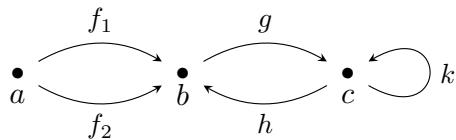
\includegraphics[keepaspectratio]{images/part001_552ae758.jpg}}

表示一个箭图，其顶点为 a、b、c，其箭为 \(f_{1}, f_{2}, g, h, k\) ，且源映射与靶映射由下式给出

\[
\begin{array}{c c c c} o (f _ {1}) = o (f _ {2}) = a & \quad o (g) = b & \quad o (h) = c & \quad o (k) = c \\ t (f _ {1}) = t (f _ {2}) = b & \quad t (g) = c & \quad t (h) = b & \quad t (k) = c. \end{array}
\]

\subsection{子箭图}

设 C 与 C′ 为箭图。若 \(\operatorname{Som}(\mathrm{C}') \subset \operatorname{Som}(\mathrm{C})\) ，\(\operatorname{Fl}(\mathrm{C}') \subset \operatorname{Fl}(\mathrm{C})\) ，且映射 \(o_{C'}\) 与 \(t_{C'}\) 分别与映射 \(o_{C}\) 与 \(t_{C}\) 在 \(\operatorname{Fl}(\mathrm{C}')\) 上相合，则称 C′ 是 C 的子箭图。此外，若 C 中源与靶都属于 \(\operatorname{Som}(\mathrm{C}')\) 的每个箭都是 C′ 的箭，则称 C′ 是 C 的全子箭图。

设 C 为箭图，\((\mathrm{C}_{i})_{i\in\mathrm{I}}\) 为 C 的子箭图族。称族 \((\mathrm{C}_{i})_{i\in\mathrm{I}}\) 的交，并记作 \(\bigcap_{i\in I}C_{i}\) ，这样的 C 的子箭图：其顶点集为 \(\bigcap_{i\in I}\mathrm{Som}(\mathrm{C}_{i})\) ，其箭集为 \(\bigcap_{i\in I}\mathrm{Fl}(\mathrm{C}_{i})\) 。

\subsection{箭图的态射}

设 C 与 C' 为箭图。从 C 到 C' 的箭图态射是一个偶 \((u,v)\) ，其中 \(u\colon\operatorname{Som}(\mathrm{C})\to\operatorname{Som}(\mathrm{C}')\) 与 \(v\colon\operatorname{Fl}(\mathrm{C})\to\operatorname{Fl}(\mathrm{C}')\) 是满足 \(o_{C'}\circ v=u\circ o_{C}\) 与 \(t_{C'}\circ v=u\circ t_{C}\) 的映射。

设 \(\varphi = (u, v)\) 为从 C 到 C' 的箭图态射。映射 \(u\) 与 \(v\) 分别记作 \(\operatorname{Som}(\varphi)\) 与 \(\operatorname{Fl}(\varphi)\) 。若 \(a\) 是 C 的顶点，则滥用记号，把 \(\varphi(a)\) 记为顶点 \(a\) 在 \(\varphi\) 下的象，我们将说 \(\varphi(a)\)

是 \(a\) 在 \(\varphi\) 下的象。类似地，若 \(f\) 是 C 的箭，则滥用记号，把 \(\varphi(f)\) 记为 C' 的箭 \(v(f)\) ，我们将说它是 \(f\) 在 \(\varphi\) 下的象。

设 C、\(C'\) 、\(C''\) 为三个箭图，\(\varphi = (u, v)\) 为从 C 到 \(C'\) 的态射，\(\varphi' = (u', v')\) 为从 \(C'\) 到 \(C''\) 的态射。则 \((u' \circ u, v' \circ v)\) 是从 C 到 \(C''\) 的态射，记作 \(\varphi' \circ \varphi\) ，称为 \(\varphi'\) 与 \(\varphi\) 的复合。

我们把 \(\mathrm{Id}_{\mathrm{C}}\) 记为从 C 到自身的态射 \((\mathrm{Id}_{\mathrm{Som}(\mathrm{C})}, \mathrm{Id}_{\mathrm{Fl}(\mathrm{C})})\) 。

设 \(\varphi\) 为从 C 到 C' 的箭图态射。为使 \(\varphi\) 是同构，必须且只需映射 \(\operatorname{Som}(\varphi)\) 与 \(\operatorname{Fl}(\varphi)\) 都是双射（参见 E, IV, 第 6 页）。

这样，若把集合 S 与 F 上的箭图结构称为两个映射 \(o, t: \mathrm{F} \to \mathrm{S}\) 的数据，就可以把箭图态射取作这个结构的态射（E, IV, 第 11 页）。

设 \(\varphi\) 为从 C 到 C' 的箭图态射。存在 C' 的唯一子箭图，其顶点集与箭集分别是 \(\mathrm{Som}(\varphi)\) 与 \(\mathrm{Fl}(\varphi)\) 的象。把它记作 \(\varphi(\mathrm{C})\) ，称为 C 在 \(\varphi\) 下的象。称 \(\varphi\) 是单射的，若映射 \(\mathrm{Som}(\varphi)\) 与 \(\mathrm{Fl}(\varphi)\) 都是单射；这时 \(\varphi\) 诱导一个从 C 到其象上的同构。

设 \(\varphi\) 与 \(\psi\) 为从 C 到 C' 的箭图态射。存在 C 的唯一子箭图，其顶点与箭分别是 C 中在 \(\varphi\) 与 \(\psi\) 下有相同象的顶点与箭。我们称之为 \(\varphi\) 与 \(\psi\) 的均衡子。

\subsection{箭图的积}

设 \((\mathrm{C}_{i})_{i\in\mathrm{I}}\) 为箭图族。令 \(S = \prod_{i\in\mathrm{I}} \mathrm{Som}(\mathrm{C}_{i})\) ，\(F = \prod_{i\in\mathrm{I}} \mathrm{Fl}(\mathrm{C}_{i})\) ，并设 o 与 t 分别为映射 \(\prod_{i\in\mathrm{I}} o_{C_{i}}\) 与 \(\prod_{i\in\mathrm{I}} t_{C_{i}}\) 。四元组 \(C = (S, F, o, t)\) 是一个箭图，称为族 \((\mathrm{C}_{i})_{i\in\mathrm{I}}\) 的积箭图。

存在唯一的箭图态射 \(pr_{i}: C \to C_{i}\) ，使得映射 \(\operatorname{Som}(\operatorname{pr}_{i})\) 与 \(\operatorname{Fl}(\operatorname{pr}_{i})\) 分别是从 \(\operatorname{Som}(C)\) 到 \(\operatorname{Som}(C_{i})\) 上与从 \(\operatorname{Fl}(C)\) 到 \(\operatorname{Fl}(C_{i})\) 上的指标 i 投影。

我们有下列泛性质：设 C' 为箭图；对任何族 \((\varphi_{i})_{i\in\mathrm{I}}\) ，其中对每个 \(i\in I\) ，\(\varphi_{i}\colon C'\to C_{i}\) 是箭图态射，存在唯一的箭图态射 \(\varphi\colon\mathrm{C}^{\prime}\to\mathrm{C}\) ，使得 \(\varphi_{i}=\mathrm{pr}_{i}\circ\varphi\) （对所有 \(i\in\mathrm{I}\) ）。

\subsection{箭图中的道路与圈}

定义 2. —— 设 C 为箭图。C 中的道路是一个序列 \(c = (a_{0}, f_{1}, a_{1}, \ldots, a_{n-1}, f_{n}, a_{n})\) ，其中 \(n\) 是整数 \(\geqslant 0\) ，\(a_{0}, \ldots, a_{n}\) 是 C 的顶点，且对 \(1 \leqslant i \leqslant n\) ，\(f_{i}\) 是 C 中连接 \(a_{i-1}\) 与 \(a_{i}\) 的箭。我们说道路 c 的长度为 \(n\) 。

设 \(c = (a_{0}, f_{1}, a_{1}, \ldots, a_{n-1}, f_{n}, a_{n})\) 为 C 中长度为 n 的道路。顶点 \(a_{0}\) 称为 c 的起点或源；顶点 \(a_{n}\) 称为 c 的终点或靶；也说 c 连接顶点 \(a_{0}\) 与顶点 \(a_{n}\) 。顶点 \(a_{i}\) （\(0 \leqslant i \leqslant n\)）称为指标 i 的顶点；箭 \(f_{i}\) （\(1 \leqslant i \leqslant n\)）称为第 i 个箭，或指标 i 的箭。长度 \(\geqslant 1\) 的道路由其箭的序列确定。

起点与终点相同的道路称为圈。长度为 0 的道路是圈，称为常值圈。

我们说道路

\[
c = (a _ {0}, f _ {1}, a _ {1}, \ldots , a _ {n - 1}, f _ {n}, a _ {n}) \text{且} c ^ {\prime} = (a _ {0} ^ {\prime}, f _ {1} ^ {\prime}, a _ {1} ^ {\prime}, \ldots , a _ {m - 1} ^ {\prime}, f _ {m} ^ {\prime}, a _ {m} ^ {\prime})
\]

在 C 中是可并列的，如果 c 的终点 \(a_{n}\) 是起点 \(a_{0}^{\prime}\) （\(c^{\prime}\) 的）。这时，序列 \((a_{0}, f_{1}, a_{1}, \ldots, a_{n-1}, f_{n}, a_{n}, f_{1}^{\prime}, a_{1}^{\prime}, \ldots, f_{m}^{\prime}, a_{m}^{\prime})\) 是 C 中的道路，记作 \(c * c^{\prime}\) ，称为 c 与 \(c^{\prime}\) 的并列道路。它连接 c 的起点与 \(c^{\prime}\) 的终点；其长度是道路 c 与 \(c^{\prime}\) 的长度之和。

\subsection{箭图的连通分支}

设 \(C = (S, F, o, t)\) 为箭图。考虑 S 上的等价关系 \(R_{C}\) ，即使得对 C 的每个箭 f 关系 \(\mathrm{R}_{\mathrm{C}}\{o(f), t(f)\}\) 成立的最细者。C 的两个顶点 a、b 对这个关系等价，当且仅当存在整数 \(n \geqslant 0\) 、C 的顶点 \(a_{0}, \ldots, a_{n}\) 与 C 的箭 \(f_{1}, \ldots, f_{n}\) ，使得 \(a_{0} = a\) ，\(a_{n} = b\) ，且对 \(1 \leqslant i \leqslant n\) ，箭 \(f_{i}\) 或者连接 \(a_{i-1}\) 与 \(a_{i}\) ，或者连接 \(a_{i}\) 与 \(a_{i-1}\) 。

这个等价关系的等价类称为 C 的连通分支。以 \(\pi_0(\mathrm{C})\) 表示 C 的连通分支所成的集。最后，若 C 至多有一个连通分支，则称 C 是连通的。

设 \(\varphi\colon\mathrm{C}\to\mathrm{C}^{\prime}\) 为箭图态射。映射 \(\operatorname{Som}(\varphi)\) 通过过渡到商，定义了一个从 \(\pi_{0}(\mathrm{C})\) 到 \(\pi_{0}(\mathrm{C}^{\prime})\) 的映射，我们把它记作 \(\pi_{0}(\varphi)\) 。

\section{图}

\subsection{图的定义}

定义 1. —— 图 \(^{(1)}\) 是一个箭图 (S, F, o, t)，带有一个 F 的对合，记作 \(f \mapsto \overline{f}\) ，它没有不动点，且满足 \(t(\overline{f}) = o(f)\) （对所有 \(f \in F\) ）。

称箭图 (S, F, o, t) 为这个图的底箭图。对这个箭图的每个箭 f，按定义有 \(\overline{\overline{f}} = f\) 、\(\overline{f} \neq f\) 与 \(t(\overline{f}) = o(f)\) 。把最后这个关系应用于箭 \(\overline{f}\) ，就得到等式 \(o(\overline{f}) = t(f)\) 。箭 \(\overline{f}\) 称为 f 的相反箭。

图的一对相反箭称为图的一条边。属于这个偶的两个箭中的每一个都称为这条边的一个定向。因此，图的箭也称为图的定向边。

若 G 与 G' 是图，从 G 到 G' 的图态射是箭图态射 \(\varphi\colon\mathrm{G}\to\mathrm{G}'\) ，它满足 \(\overline{\varphi(f)}=\varphi(\overline{f})\) （对 G 的每个箭 \(f\) ）。

设 G 与 G' 为图；若 G' 是子箭图且 Fl(G') 的对合是 Fl(G) 的对合的限制，则称 G' 是 G 的子图。

\subsection{图的定向}

设 G 为图。G 的一个定向是 G 的箭集的一个子集 A，满足 \(A \cap \overline{A} = \varnothing\) 且 \(A \cup \overline{A} = \mathrm{Fl}(G)\) 。

带有一个定向的图称为定向图。

设 G 为定向图，A 为其定向；G 的定向子图是子图 \(G'\) （G 的），带有定向 \(A' = \mathrm{Fl}(G') \cap A\) 。

设 (G, A) 与 (G', A') 为定向图。从 (G, A) 到 (G', A') 的定向图态射是图态射 \(\varphi\colon G \to G'\) ，满足 \(\operatorname{Fl}(\varphi)(A) \subset A'\) 。

\subsection{定向图与箭图}

设 G 为图，\((S,F,o,t)\) 为其底箭图，A 为 G 的一个定向。则 \((S,A,o\mid A,t\mid A)\) 是一个箭图，称为与定向图 \((G,A)\) 伴随的箭图。

反之，设 \(C = (S, F, o, t)\) 为箭图。令 \(\widetilde{F} = F \times \{-1, 1\}\) ，并设 \(\widetilde{o}, \widetilde{t}\) 为由下式定义的从 \(\widetilde{F}\) 到 S 的映射

\[
\begin{array}{l l} \widetilde {o} (f, 1) = o (f) & \qquad \qquad \widetilde {o} (f, - 1) = t (f) \\ \widetilde {t} (f, 1) = t (f) & \qquad \qquad \widetilde {t} (f, - 1) = o (f), \end{array}
\]

对每个 \(f \in \mathrm{F}\) 。于是，\(\widetilde{\mathrm{C}} = (\mathrm{S}, \widetilde{\mathrm{F}}, \widetilde{o}, \widetilde{t})\) 赋有对合 \((f, \varepsilon) \mapsto (f, -\varepsilon)\) （\(\widetilde{\mathrm{F}}\) 的），是一个图，称为与箭图 C 伴随的图。集 \(\mathrm{A} = \mathrm{F} \times \{1\}\) 是这个图的一个定向。称 \((\widetilde{\mathrm{C}}, \mathrm{A})\) 为与箭图 C 伴随的定向图。

若 \(f\) 是 C 的箭，也说 \((f,1)\) 是 \(\widetilde{C}\) 的与 \(f\) 伴随的定向边，且偶 \(\{(f,1),(f,-1)\}\) 是 \(\widetilde{C}\) 的与 \(f\) 伴随的边。

若 C' 是 C 的子箭图，则定向图 \(\widetilde{C}'\) 是 \(\widetilde{C}\) 的定向子图。

存在唯一的箭图态射 \(\varphi\) （从 C 到 \(\widetilde{\mathrm{C}}\) 的底箭图），使得 \(\varphi(f) = (f,1)\) （对 C 的每个箭 \(f\) ）；它是从 C 到与定向图 ( \(\widetilde{\mathrm{C}}\) , A) 伴随的箭图上的同构。

\subsection{树}

当谈到图的道路或连通分支时，指的是底箭图的道路或连通分支。图的两个顶点属于同一连通分支，当且仅当存在连接它们的道路。

设 G 为图。若 \(c = (a_{0}, f_{1}, a_{1}, \ldots, f_{n}, a_{n})\) 是 G 中的道路，则序列 \(\overline{c} = (a_{n}, \overline{f_{n}}, \ldots, a_{1}, \overline{f_{1}}, a_{0})\) 是 G 中的道路，称为 c 的相反道路。设 c 与 \(c'\) 是 G 中可并列的道路；则 \(\overline{c'}\) 与 \(\overline{c}\) 可并列，且有 \(\overline{c * c'} = \overline{c'} * \overline{c}\) 。

若 c 中没有一对相邻的箭是相反的，则称 G 中的道路 c 是无回溯的。设 \(c = (a_{0}, f_{1}, \ldots, f_{n}, a_{n})\) 为 G 中连接 \(a_{0}\) 与 \(a_{n}\) 的道路。若对满足 \(1 \leqslant i < n\) 的整数 i，箭 \(f_{i}\) 与 \(f_{i+1}\) 相反，则 \((a_{0}, f_{1}, \ldots, a_{i-1}, f_{i+2}, \ldots, f_{n}, a_{n})\) 是 G 中连接 \(a_{0}\) 与 \(a_{n}\) 的道路，其长度严格小于道路 c 的长度。由归纳法，因此存在 G 中连接 \(a_{0}\) 与 \(a_{n}\) 的无回溯道路。

定义 2. —— 森林是这样的图：其中每条无回溯的圈都是常值圈。树是连通的森林。

命题 1. —— 设 G 为图。G 的每个森林都含于 G 的一个极大森林中；特别地，存在 G 的极大森林。

为使 G 的森林是极大的，必须且只需其顶点集等于 G 的顶点集，且其连通分支就是 G 的连通分支。

设 \(A_{0}\) 为 G 的森林。G 的森林所成的集，赋有序关系“A 是 B 的子图”后，是归纳的。因此，存在 G 的极大森林，\(A_{0}\) 是它的子图（E, III, 第 21 页, 推论 1）。

以 \(\operatorname{Som}(G)\) 为顶点集、箭集为空的 G 的子图是 G 的森林。因此存在 G 的极大森林。

设 A 为 G 的极大森林。我们证明 A 与 G 有相同的顶点集。以 \(\operatorname{Som}(G)\) 为顶点集、以 \(\operatorname{Fl}(A)\) 为箭集的 G 的子图是一个森林，且 A 是它的子图。于是有 \(\operatorname{Som}(A) = \operatorname{Som}(G)\) 。

现在证明 A 与 G 有相同的连通分支。由于 A 的每个箭都是 G 的箭，A 的每个连通分支含于 G 的一个连通分支。既然 A 与 G 有相同的顶点集，只需证明 G 中处于同一连通分支的两个顶点也处于 A 的同一连通分支。若不然，关系 \(R_{A}\) （“处于 A 的同一连通分支”）严格细于关系 \(R_{G}\) ，且存在 G 的两个顶点，它们不处于 A 的同一连通分支，但却被 G 的一个箭 f 连接。设 B 为 G 的定向子图，其顶点集为 \(\operatorname{Som}(G)\) ，箭集为 \(\mathrm{Fl(A)} \cup \{f, \overline{f}\}\) 。我们来证明 B 是 G 的森林。设 \(c = (a_{0}, f_{1}, \ldots, f_{n}, a_{n})\) 为 B 中长度最小的非常值无回溯圈。由于 A 是森林，圈 c 不是 A 中的圈。设 i（相应地，j）为 \(\{0, \ldots, n\}\) 中使 \(a_{0}\) 与 \(a_{i}\) （相应地，\(a_{j}\) 与 \(a_{n}\) ）不处于 A 的同一连通分支的最小（相应地，最大）整数。这意味着箭 \(f_{i}\) 与 \(f_{j+1}\) 是 B 中与边 \(\{f, \overline{f}\}\) 伴随的定向箭，且它们相反。由于圈 c 无往返，\(f_{i+1} \neq \overline{f_{i}}\) ，因此 \(i \neq j\) ，而道路 \((a_{i}, f_{i+1}, a_{i+1}, \ldots, f_{j}, a_{j})\) 是 B 中长度 < n 的非常值无回溯圈，与 c 长度最小的假设矛盾。由此推出 B 是森林。这与 A 是 G 的极大森林的假设矛盾。

现设 A 为 G 的森林，满足 \(\mathrm{Som}(\mathrm{A}) = \mathrm{Som}(\mathrm{G})\) 与 \(\pi_{0}(\mathrm{A}) = \pi_{0}(\mathrm{G})\) 。我们来证明它是 G 的极大森林。只需证明：若 \(f \notin \mathrm{Fl}(\mathrm{A})\) ，则 G 的以 \(\mathrm{Som}(\mathrm{G})\) 为顶点集、以 \(\mathrm{Fl}(\mathrm{A}) \cup \{f, \overline{f}\}\) 为箭集的子图 B 不是森林。按假设，点 \(o(f)\) 与 \(t(f)\) 处于 A 的同一连通分支；因此存在 A 中连接 \(o(f)\) 与 \(t(f)\) 的无回溯道路 c。于是道路 \(c * \overline{f}\) 是 B 中无回溯且非常值的圈，这表明 B 不是森林。

推论. —— 连通图的极大森林是它的极大树。

注 1. —— 在 LIE, IV, 第 33 页附录中，组合图的概念定义为偶 (A, S)，其中 S 是一个集合，

而 A 是 \(\mathfrak{P}(S)\) 的由二元集组成的子集；S 的元素称为顶点，A 的元素称为边，且两个顶点 \(x\) 与 \(y \in S\) 称为相连的，如果 \(\{x, y\}\) 是一条边。

对这样的组合图 \(\Gamma = (\mathrm{A},\mathrm{S})\) ，伴随一个图 G，其顶点集为 S，箭集 \(\widetilde{\mathrm{A}}\) 是 \(\mathrm{S}^2\) 中由相连顶点的偶所组成的子集，其源映射与靶映射分别与 \(\mathrm{S}^2\) 到 S 的第一、第二投影相合，而对合 \(f\mapsto \overline{f}\) 由 \(\widetilde{\mathrm{A}}\) 上的映射 \((x,y)\mapsto (y,x)\) （\(\mathrm{S}^2\) 到自身的）的限制给出。把 G 的边 \(\{f,\overline{f}\}\) 映为集合 \(\{o(f),t(f)\}\) 的映射是从 G 的边集到组合图 \(\Gamma\) 的边集上的双射。

反之，每个使得每个箭的源与靶不同、且箭由其源与靶确定的图，都具有这种形式。

读者可以验证，组合图的连通性、树或森林的概念，与与之伴随的图的相应概念一致。

\section{群胚}

\subsection{范畴}

定义 1. —— 设 C 为箭图。以 J 表示 C 中箭的偶 \((f,g)\) （满足 \(t(f)=o(g)\) ）所成的集。C 上的一个合成律是这样的映射 \(m:J\to\mathrm{Fl}(\mathrm{C})\) ：对每个偶 \((f,g)\in\mathrm{J}\) ，箭 \(m(f,g)\) 的起点是 f 的起点，其靶是 g 的靶。

设 C 为带有一个合成律 \(m\) 的箭图。两个箭 \(f\) 与 \(g\) （满足 \(t(f) = o(g)\) ）称为可复合的；箭 \(m(f, g)\) 称为它们的复合，或它们的乘积，常记作 \(f \cdot g\) ，甚至记作 \(fg\) 。

对 C 的每个顶点 \(a\) ，集合 \(\mathrm{C}_{a,a} = \mathrm{Fl}_{a,a}(\mathrm{C})\) 赋有由 \(m\) 过渡到子集而得的映射后，是一个群原（A, I, 第 1 页, 定义 1）。

C 的箭的族 \((f_{i})_{i\in\mathrm{I}}\) ，以有限非空全序集 I 为指标集，若对 I 的每对相邻元素 \((i,j)\) ，箭 \(f_{i}\) 与 \(f_{j}\) 可复合，则称该族是可复合的。这样的族的乘积 \(\prod_{i\in\mathrm{I}}f_{i}\) 由对 I 的基数用归纳法定义如下（参见 A, I, 第 3 页）：

\begin{enumerate}
\def\labelenumi{(\roman{enumi})}
\item
  若 I 只有一个元素 \(\omega\) ，则 \(\prod_{i\in I}f_i = f_\omega\) ；
\item
  若 I 至少有两个元素且 \(\omega\) 是 I 的最小元素，则令 \(\prod_{i\in I}f_i = f_\omega \cdot \prod_{i\in I - \{\omega \}}f_i\) 。
\end{enumerate}

合成律 \(m\) 称为结合的，若 \(f \cdot (g \cdot h) = (f \cdot g) \cdot h\) （对 C 的箭的每个可复合三元组 \((f, g, h)\) ）。当律 \(m\) 结合时，序列 \((f_1, \ldots, f_n)\) （\(n\) 个可复合箭的，其中 \(n\) 为整数 \(\geqslant 1\) ）的乘积记作 \(f_1 f_2 \ldots f_n\) 。

设 \(a\) 为 C 的顶点。称箭 \(e \in \mathrm{C}_{a,a}\) 是 \(m\) 在 \(a\) 处的单位元，若 \(ef = f\) （对每个箭 \(f\) ，以 \(a\) 为源的），且 \(ge = g\) （对每个箭 \(g\) ，以 \(a\) 为终点的）。\(m\) 在 \(a\) 处至多有一个单位元：若 \(e\) 与 \(e'\) 是两个单位元，则有 \(e' = ee' = e\) 。当这样的单位元存在时，常记作 \(e_a\) ；它这时是群原 \(\mathrm{C}_{a,a}\) 的单位元（A, I, 第 12 页）。

定义 2. —— 范畴是带有一个结合合成律的箭图，且在每个顶点处存在单位元。

例. —— 1) 设 C 为箭图。以 Ch(C) 表示 C 中道路所成的集，以 o: Ch(C) → Som(C)、t: Ch(C) → Som(C) 表示把道路映为其起点与终点的映射。四元组 \(\Omega_{\mathrm{C}} = (\mathrm{Som}(\mathrm{C}), \mathrm{Ch}(\mathrm{C}), o, t)\) 是一个箭图。给它赋予由道路的衔接定义的合成律。这个合成律是结合的；对 C 的每个顶点 a，以 a 为起点的常值圈 \(e_a = (a)\) 是 a 处的单位元。这样，\(\Omega_{\mathrm{C}}\) 是一个范畴。称之为箭图 C 的道路范畴。

\begin{enumerate}
\def\labelenumi{\arabic{enumi})}
\setcounter{enumi}{1}
\tightlist
\item
  设 \(\Sigma\) 为比集合论更强的理论 \(\mathcal{T}\) 中的一种结构，\(\sigma\{x,y,s,u\}\) 为 \(\mathcal{T}\) 中满足 E, IV, 第 11 页的条件 (MO \(_{\text{I}}\) )、(MO \(_{\text{II}}\) ) 与 (MO \(_{\text{III}}\) ) 的项。设 S 为集合；假设 S 的每个元素都是偶 \((x,s)\)，其中 \(x\) 是集合，\(s\) 是种 \(\Sigma\) 的结构（在 \(x\) 上的）。设 F 为这样的映射 \(f\) 所成的集：存在 S 中的 \((x,s)\) 与 \((y,t)\) ，使 \(f\) 是一个 \(\sigma\) -态射，从 \(x\) （赋有结构 \(s\) 的）到 \(y\) （赋有结构 \(t\) 的）；这时令 \(o(f) = (x,s)\) 与 \(t(f) = (y,t)\) 。赋有由 \(m(f,g)=g\circ f\) 给出的合成律后，箭图 (S,F,o,t) 是一个范畴。在这种语境下，S 的元素更常称为对象。
\end{enumerate}

设 C 为范畴。

对 C 的每个顶点 \(a\) ，集合 \(\mathrm{C}_{a,a}\) 赋有合成律 \((f,g)\mapsto fg\) 后，是以 \(e_a\) 为单位元的幺半群。

称 C 的箭 \(f\) 是可逆的，若存在 C 的箭 \(g\) ，使得 \(o(g) = t(f)\) 、\(t(g) = o(f)\) ，且 \(fg\) 与 \(gf\) 分别是 \(o(f)\) 与 \(t(f)\) 处的单位元。这样的箭 \(g\) 是唯一的（若 \(fg = e_{o(f)}\) 且 \(g'f = e_{t(f)}\) ，则有 \(g = e_{t(f)}g = (g'f)g = g'(fg) = g'e_{o(f)} = g'\) ），称为 \(f\) 的逆；可逆箭 \(f\) 的逆记作 \(f^{-1}\) 。

\subsection{函子}

定义 3. —— 设 C 与 C' 为范畴。从 C 到 C' 的函子是箭图态射 \(\varphi\colon\mathrm{C}\to\mathrm{C}'\) ，满足 \(\varphi(fg)=\varphi(f)\varphi(g)\) （对 C 的每对可复合箭 \((f,g)\) ）。

设 C 与 C' 为范畴，\(\varphi\colon\mathrm{C}\to\mathrm{C}'\) 为函子。设 \(f\) 为 C 的箭，\(a\) 为其起点，\(b\) 为其靶；则 \(\varphi(f)\) 是 C' 的箭，起点为 \(\varphi(a)\) ，靶为 \(\varphi(b)\) 。

设 C、C'、C'' 为范畴，\(\varphi\colon\mathrm{C}\to\mathrm{C}'\) 与 \(\varphi'\colon\mathrm{C}'\to\mathrm{C}''\) 为函子。则 \(\varphi'\circ\varphi\) 是函子。

设 C 为范畴。则箭图态射 \(Id_{C}\) 是函子。

设 \(\varphi\colon\mathrm{C}\to\mathrm{C}^{\prime}\) 为函子。为使 \(\varphi\) 是同构，必须且只需映射 \(\operatorname{Som}(\varphi)\) 与 \(\operatorname{Fl}(\varphi)\) 都是双射。

这样，若把集合 S 与 F 上的范畴结构称为这些集合上的箭图结构与一个在每个顶点处存在单位元的结合合成律的数据，就可以把函子取作这个范畴结构的态射（E, IV, 第 11 页）。

\subsection{群胚}

定义 4. —— 群胚是每个箭都可逆的范畴。

设 G 为群胚，a 为 G 的顶点。幺半群 \(G_{a,a}\) 是一个群，记作 \(G_{a}\) ，称为 G 在 a 处的迷向群。

设 \(a\) 与 \(b\) 为 G 的顶点，\(f \in \mathrm{G}_{a,b}\) 为连接 \(a\) 与 \(b\) 的箭。映射 \(g \mapsto fgf^{-1}\) 是从 \(\mathrm{G}_b\) 到 \(\mathrm{G}_a\) 的群同构，记作 \(\operatorname{Int}(f)\) 。若 \(f\) 与 \(f'\) 是 G 的可复合箭，则有 \(\operatorname{Int}(ff') = \operatorname{Int}(f) \circ \operatorname{Int}(f')\) 。同构 \(\operatorname{Int}(f)\) 的逆是同构 \(\operatorname{Int}(f^{-1})\) 。

群胚态射 \(\varphi\colon G\to G'\) 是范畴态射。此外，\(\varphi\) 是群胚同构当且仅当它是范畴同构。

设 \(\varphi\colon\mathrm{G}\to\mathrm{G}^{\prime}\) 为群胚态射。对 G 的每个顶点 \(a\) ，映射 \(f\mapsto\varphi(f)\) （从 \(\mathrm{G}_{a}\) 到 \((\mathrm{G}^{\prime})_{\varphi(a)}\) 的）是群同态，记作 \(\varphi_{a}\) 。特别地，有 \(\varphi(e_{a})=e_{\varphi(a)}\) 。

对 G 的每个箭 \(f\) ，\(\varphi(f^{-1})\) 是 \(\varphi(f)\) 的逆。若 \(f\) 是 G 中连接顶点 \(a\) 与顶点 \(b\) 的箭，则对每个元素 \(g \in \mathrm{G}_b\) ，有关系 \(\operatorname{Int}(\varphi(f))(\varphi(g)) = \varphi(\operatorname{Int}(f)(g))\) 。

\subsection{群胚的轨道}

设 G 为群胚。G 的底箭图的连通分支称为 G 的轨道。G 的轨道所成的集记作 \(\mathrm{Orb}(\mathrm{G})\) ；若 \(\varphi: G \to G'\) 是群胚态射，则映射 \(\pi_{0}(\varphi)\) （由 \(\varphi\) 过渡到伴随图的连通分支而得的）通常记作 \(\mathrm{Orb}(\varphi)\) ，称为由 \(\varphi\) 过渡到轨道而得的映射。

恰有一个轨道的群胚称为传递的。若 G 是传递群胚，则诸群 \(G_{a}\) （对 \(a \in \text{Som}(G)\) ）彼此同构。若群胚 G 是传递的，且诸迷向群 \(G_{a}\) 都缩为各自的单位元，则称群胚 G 是单传递的。

命题 1. —— 设 G 为群胚。关系“存在 G 的箭连接 a 与 b”是 G 的顶点集上的等价关系，其等价类即 G 的轨道。

设 \(a\) 、\(b\) 、\(c\) 为 G 的顶点。我们有 \(e_a \in \mathrm{G}_{a,a}\) ；若 \(f \in \mathrm{G}_{a,b}\) ，则 \(f^{-1} \in \mathrm{G}_{b,a}\) ；若 \(f \in \mathrm{G}_{a,b}\) 且 \(g \in \mathrm{G}_{b,c}\) ，则有 \(fg \in \mathrm{G}_{a,c}\) 。这表明所指的关系是自反的、对称的且传递的；因此是等价关系。第二个断言由箭图连通分支的定义得出。

\subsection{群胚的例子}

\begin{enumerate}
\def\labelenumi{\arabic{enumi})}
\item
  设 G 为群。以 \(\mathcal{G}\) 表示这样的箭图：其顶点集缩为单个元素，其箭集为 G。\(\mathcal{G}\) 赋有由 G 的合成律诱导的合成律后，是一个群胚，称为与群 G 伴随的群胚。
\item
  设 X 为集合。设 G 为箭图 \((\mathrm{X}, \mathrm{X} \times \mathrm{X}, \mathrm{pr}_{1}, \mathrm{pr}_{2})\) ；在 G 上定义合成律：令 \((x, x') \cdot (x', x'') = (x, x'')\) （若 \(x, x', x''\) 是 X 的元素）。这个律是结合的；对每个 \(x \in X\) ，\((x, x)\) 是 x 处的中性元；箭 \((x, x')\) 的逆是箭 \((x', x)\) 。这样定义的群胚称为集合 X 的偶对群胚。若 X 非空，它是单传递的。
\item
  设 X 与 S 为集合，\(p \colon \mathrm{X} \to \mathrm{S}\) 为映射。对 \(a \in \mathrm{S}\) ，记 \(\mathrm{X}_a = p^{-1}(a)\) 。对 S 中的 \(a\) 与 \(b\) ，设 \(\mathrm{G}_{a,b}\) 为集 \(\mathcal{B}(\mathrm{X}_a; \mathrm{X}_b)\) （从 \(\mathrm{X}_a\) 到 \(\mathrm{X}_b\) 的双射所成的），并设 G 为诸集 \(\mathrm{G}_{a,b}\) 的不交并。设 \(o\) 与 \(t\) 为从 G 到 S 的映射，使得 \(o(f) = a\) 与 \(t(f) = b\) （对每个元素 \(f \in \mathrm{G}_{a,b}\) ）。四元组 \((\mathrm{S}, \mathrm{G}, o, t)\) 是一个箭图。给它赋予由 \(m(f, g) = g \circ f\) （若 \(f \in \mathcal{B}(\mathrm{X}_a; \mathrm{X}_b)\) 且 \(g \in \mathcal{B}(\mathrm{X}_b; \mathrm{X}_c)\) ，其中 \(a, b, c\) 是 S 的元素）定义的合成律。这是一个群胚；记作 \(\mathcal{B}(\mathrm{X}, p)\) ，称为 X 相对于 \(p\) 的置换群胚。
\item
  设 \((\mathrm{G}_{i})_{i\in\mathrm{I}}\) 为群胚族。以 G 表示诸底箭图族的积箭图；对每个 \(i\in I\) ，设 \(pr_{i}\colon G\to G_{i}\) 为典范箭图态射。G 上存在唯一的合成律，使 G 成为群胚，且对每个 \(i \in I\) ，\(\mathrm{pr}_i\) 是群胚态射。设 \(f = (f_i)_{i \in I}\) 与 \(g = (g_i)_{i \in I}\) 为 G 的箭；它们可复合，当且仅当箭 \(f_i\) 与 \(g_i\) 可复合（对 \(i \in I\) ）。这时有 \(fg = (f_i g_i)_{i \in I}\) 。
\end{enumerate}

箭图 G 赋有这个合成律后，称为族 \((\mathrm{G}_{i})_{i\in\mathrm{I}}\) 的积群胚。它满足下列泛性质：对每个群胚 \(G'\) 与每个族 \((\varphi_{i})_{i\in\mathrm{I}}\) （其中 \(\varphi_{i}\) 是从 \(G'\) 到 \(G_{i}\) 的群胚态射），存在唯一的群胚态射 \(\varphi: G'\to G\) ，使得 \(\varphi_{i}=\operatorname{pr}_{i}\circ\varphi\) （对所有 \(i\in I\) ）。

\begin{enumerate}
\def\labelenumi{\arabic{enumi})}
\setcounter{enumi}{4}
\tightlist
\item
  设 \(((\mathrm{G}_{i})_{i\in\mathrm{I}},(\varphi_{i,j})_{i\prec j})\) 为群胚的归纳系，以右过滤预序集 \((\mathrm{I},\prec)\) 为指标集，其中 \(\varphi_{i,j}\) 是群胚态射。设 G 为这样的箭图：其顶点集为 \(\varinjlim_{i}\operatorname{Som}(\mathbf{G}_{i})\) ，箭集为 \(\varinjlim_{i}\operatorname{Fl}(\mathbf{G}_{i})\) ，源映射与靶映射分别为映射 \(\varinjlim_{i}o_{G_{i}}\) 与 \(\varinjlim_{i}t_{G_{i}}\) 。诸 \(G_{i}\) 的合成律在 G 上诱导一个合成律，使 G 成为群胚（参见 A, I, 第 114 页）。典范映射 \(\operatorname{Som}(\mathbf{G}_{i})\to\operatorname{Som}(\mathbf{G})\) 与 \(\operatorname{Fl}(\mathbf{G}_{i})\to\operatorname{Fl}(\mathbf{G})\) 定义了一个群胚态射 \(\varphi_{i}\) （从 \(G_{i}\) 到 G 的）。若 i、j 是 I 中满足 \(i\prec j\) 的元素，则有 \(\varphi_{j}\circ\varphi_{i,j}=\varphi_{i}\) 。群胚 G 称为群胚族 \(G_{i}\) 的归纳极限，记作 \(\varinjlim_{i}G_{i}\) 。它满足下列泛性质：对每个群胚 H 与每个族 \((\psi_{i})_{i\in\mathrm{I}}\) （其中对 \(i\in I\) ，\(\psi_{i}:G_{i}\to H\) 是群胚态射，并且 \(\psi_{j}\circ\varphi_{i,j}=\psi_{i}\) 对 I 的元素的每对 \((i,j)\) （满足 \(i\prec j\) ）成立），存在唯一的群胚态射 \(\psi:G\to H\) 使得 \(\psi_{i}=\psi\circ\varphi_{i}\) 。
\end{enumerate}

关于当不假设集 I 右过滤时满足这个泛性质的群胚的存在性，参见 II, 第 228 页, 习题 3。
